% Copyright (c) 2008-2009 solvethis
% Copyright (c) 2010-2011 Casper Ti. Vector
% Public domain.

\documentclass[UTF8]{pkuthss}
% 使得打字机粗体可以被使用。
\usepackage{lmodern}
% 产生 originauth.tex 里的 \square。
\usepackage{amssymb}
% 提供 Verbatim 环境和 \VerbatimInput 命令。
\usepackage{fancyvrb}
% 提供数学公式
\usepackage{amsmath}
% 提供theoremstyle
\usepackage{amsthm}
% 提供伪代码
\usepackage{algorithm}  
\usepackage{algpseudocode}
% 提供图片排版
\usepackage{graphicx}
\usepackage{subcaption}
% 提供表格支持
\usepackage{multirow}

\usepackage{verbatim}
% 设定图片路径
\graphicspath{{./img/}}
% pkuthss 文档模版的版本。
\newcommand{\docversion}{v1.3 beta1}

\newcommand{\mycite}[1]
{\citeauthor{#1}\parencite{#1}
}

%
\usepackage{appendix}
% 参考文献格式。
\bibliographystyle{ref/chinesebst-mod}
% 设定文档的基本信息。
\pkuthssinfo{
	cthesisname={研究生毕业论文},ethesisname={Undergraduate Thesis},
	ctitle={机器学习在地震紧急预警系统震级预估中的应用},
	etitle={Application of Machine Learning to Magnitude Estimation in Earthquake Emergency Prediction System},
	cauthor={胡安冬},
	eauthor={Andong Hu},
	studentid={1601210232},
	date={二〇一九年六月},
	school={地球与空间科学学院},
	cmajor={地球物理系},emajor={Geophysics},%direction={震源动力学},
	cmentor={张海明\ 副教授},ementor={Associate Prof.\ Haiming Zhang},
    ckeywords={地震紧急预警; 震级预估; 机器学习; 深度学习},
	ekeywords={Earthquake early warning; Magnitude estimation; Machine learning; Deep learning},
}

% 定义和例子
\theoremstyle{definition}
\newtheorem{example1}{例}
\newtheorem{example2}{例}
\newtheorem{realistic-tra}{定义}
\newtheorem{tra-record}[realistic-tra]{定义}
\newtheorem{tra-data-set}[realistic-tra]{定义}
\newtheorem{same-real-tra}[realistic-tra]{定义}
\newtheorem{tra-matching}[realistic-tra]{定义}

% 算法
\floatname{algorithm}{算法}
\renewcommand{\algorithmicrequire}{\textbf{输入:}}  
\renewcommand{\algorithmicensure}{\textbf{输出:}}  


\begin{document}
	% 以下为正文之前的部分。
	\frontmatter

	% 自动生成标题页。
	\maketitle
	% 版权声明。
	\include{chap/copyright}
	% 中英文摘要。
	% Copyright (c) 2008-2009 solvethis
% Copyright (c) 2010-2011 Casper Ti. Vector
% Public domain.

\begin{cabstract}
\indent 地震预警是地震减灾工作的重要途径,而震级预估是整个地震紧急预警系统中重要且较为困难的一个环节。目前,世界上多个国家和地区都已建立了各自的地震预警系统,并且形成了特征频率(~$\tau_{p}$~和~$\tau_{c}$~等)相关和特征振幅($P_{d}$等)相关的两类震级紧急预警的方法,但各有局限性。本文在已有的方法和理论基础上,运用机器学习算法,将日本KIK和KNET台网从2015至2017年所记录到的843条地震目录,55426条记录作为全数据集,设计、训练出一套用于常见震级范围的机器学习震级预估模型。与已有方法的预估结果相比,机器学习方法不仅使预估的整体误差和方差下降,同时多台联合评估单一地震事件的截面方差也更低。本研究的结果显示了机器学习算法在震级紧急预估问题上具有较广阔的应用前景,同时也为较为复杂的深度学习类算法框架下端到端模型提供了实践基础和研究可能。
\end{cabstract}

\begin{eabstract}
\indent Earthquake early warning (EEW) is an important way for earthquake disaster reduction, and magnitude estimation is an important and difficult part of the entire EEW system. Nowadays, many countries and regions around the world have established their own EEW systems, and two types of magnitude emergency warning methods, characteristic frequency ((~$\tau_{p}$~and~$\tau_{c}$~, etc.) and characteristic amplitude ($P_{d}$ and others), have be presented. Based on the existing methods and theories, we applied the machine learning algorithm to 55,426 records for 843 earthquakes recorded by the KIK and KNET networks in Japan from 2015 to 2017. By using these records as a full data set, a set of machine learning magnitude prediction models have been designed and trained for common magnitude ranges. Compared with the estimated results of the existing methods, the machine learning method may reduce not only the estimated overall error and variance, but also the cross-sectional variance of multiple joint seismic events. The results of this study show that machine learning algorithm has a broad application prospect in earthquake magnitude emergency estimation, and provides a practical basis and research possibilities for end-to-end model of more complex deep learning algorithm framework as well.
\end{eabstract}


	% 自动生成目录。
	\tableofcontents

	% 以下为正文。
	\mainmatter

	% 绪言。
	% \include{chap/introduction}
	
	% 各章节。
	% Copyright (c) 2008-2009 solvethis
% Copyright (c) 2010-2011 Casper Ti. Vector
% Public domain.

\chapter{引言}
\section{研究背景}
\indent 我国是遭受地震灾害最为严重的国家之一。在过去的20世纪里,因大陆地震而造成死亡的人数中我国超过60万人,占全球总人数一半以上(金星等, 2003, 2012)。与此同时,随着近海陆地城市化进程的推进,我国60\%的百万人口城市都位于高烈度区域,其中包括全国23个省会城市,地震灾害对这些地区人民的生命和财产构成严重威胁(张红才等, 2012)。为了减少地震灾害造成的生命财产损失,地震预警 (EEW) 系统应运而生。它合理地利用城市和地震源之间的空间关系,同时配合人民群众接受适当的训练以响应地震警报信息,成为减少地震灾害的有效手段 (Allen et al., 2007)。\\
\indent EEW系统对即将发生强烈震动的城市区域发出预警,在破坏性强的S波部分到达之前通常具有几秒到几十秒的预警时间,这个宝贵的时段可为各种关键设施预设紧急措施:例如紧急制动正在运行的高铁和动车,以避免潜在的脱轨;关闭天然气管道,以最大限度地减少火灾危险;紧急备份与关闭计算机等设施,以避免重要数据库丢失 (Kamigaichi et al., 2009; Allen et al., 2007; Iglesias et al., 2007)。EEW系统包括实时地震定位、实时震级预估、预警目标区烈度估计和预警信息发布四个主要部分。目前已经有成熟的方法进行地震定位和预警信息发布。但作为决定EEW系统好坏的重要环节的实时震级预估,仍存在着诸多难点:首先,大地震震级难以准确测定。较大的地震都是由多个断层破裂组成,单次断层破裂过程也十分复杂;其次,在EEW有时效性的要求下,短时窗内观测到信息少,常用的震级计算方法会在6.5级左右产生明显的震级饱和 (Kanamori et al., 2009);此外,发震断层走向和倾向等参数对地面运动分布也会产生显著影响,但这些震源参数难以实时得到。\\
\indent 已有的解决方案在很多方面还有待提高。例如,在常见震级范围内漏报和误报情况出现频率较高;为了得到稳定的预估结果,需要的台站较多;仍无法解决震源参数高效实施获得等。单台站震级预估方法因其简单和快速的特点成为当前震级紧急预估的主流方法,但无论是以$\tau_{p}$和$\tau_{c}$ (Nakamura et al., 1993; Kanamori et al., 2005) 为核心的特征频率相关方法,还是以$\mathrm{P}_{\mathrm{d}}$(Wu et al., 2007; Kanamori et al., 2008, 2009) 为核心的振幅相关方法,都只使用了地震台站的垂直分量记录,导致信息极大的浪费。由于两类方法的出发点不同,各自具有一定的局限性,比如$\tau_{c}$类方法在实践中被证实在部分地区效果不好(Horiuchi et al., 2006),而$\mathrm{P}_{\mathrm{d}}$类方法对于长破裂时间的震源更容易震级饱和 (Zollo et al., 2006)。以上研究结果表明,以单一特征为核心的震级预估算法不够强健,促使了相对应的多特征间相容性的研究(张红才等, 2017)。另一方面,如果在EEW系统中加入实时震源参数检测,则会使得准确性与所用时间同时增加 (Heaton et al., 1985; Allen,2006)。例如,在意大利的Preto系统中,预先根据历史地震和对应断层预设数据库,发震后从数据库中自动匹配断层参数 (Weber et al., 2007),但在时效上仍难以达到实时预警的要求。\\
\section{本文研究的意义}
\indent 本文针对EEW系统的实时震级预估问题,采用机器学习类算法解决和优化以上提到的诸多问题。一方面,高密度地震台网记录的地震数据给需求巨量训练数据的机器学习算法提供了训练的可能性;另一方面,机器学习算法可以充分利用台站记录的完整数据,避免了已有算法中只利用单一分量造成的信息浪费。此外,考虑到不同地区断层有不同特点,机器学习算法能自动训练出最适合当地的震级预测模型,这使得模型可以获得最佳适应断层模型和震源参数的影响。本研究显示出新模型预估震级的能力显著优于已有方法,表明机器学习算法在震级紧急预估问题上具有较广阔的应用前景,同时也为较为复杂的深度学习类算法框架下端到端模型提供了实践基础和研究可能。\\
\indent 同时传统震级预估方法对于低信噪比数据的处理能力较低、抗噪声干扰差。以目前两类主流EEWs所使用的震级预估模块的算法特点,都还不能良好处理大型地震后频繁出现的余震。但事实上大型破坏地震之后的余震危害是巨大的,根据中国地震台网中心统计,2008年汶川地震主震发生后的三个月内,共发生6级以上的余震6次,5级至6级的余震30次。(陈九辉等,2009)。这些高强度余震很多时候都会被主震或其他与余震的尾波所干扰,导致使用传统方法在预估余震震级上往往会有较大的偏差。而机器学习CNN类算法在滤波抗噪方面有独特结构带来的优势,即使台站信息被噪音或主震尾波淹没仍可以在一定程度上,从中剥离出需要紧急预估的余震震级。\\
\section{本文的内容}
\indent 除去本章节外本文剩余共分为四章。其中第二章为传统震级预估方法的简介,先从物理学本质上讨论了震级预估的可行性,随后探究了特征频率和特征幅值两类主要传统震级预估法的实现方式和其内涵。在第三章详细介绍所设计的机器学习类震级预估方法,并针对地震学问题对如何进行数据集划分和模型评估进行了讨论。在第四章中使用日本地区的密集台网数据对两类机器学习类模型进行训练,将训练好的模型与传统方法从多方面进行了性能比较。在第五章对本文工作进行了总结,同时对仍待未解决的问题和有望完成的工作进行了展望。\\
	
\chapter{传统震级预估方法简介}

\section{预估震级的可能性}

\indent 能够由初始破裂信息估计出整个地震的规模是预估震级可行的基本前提。目前学术界对于这个问题仍没有一致性的认识。持否定态度的学者认为破裂过程在时序上是不可预测,即使用已得到的地震台信息只能评估目前的地震释放的能量但不能预估整个断层破裂结束所释放的能量大小(Mori, 1996; Kilb et al, 1999),。但仍有已有多种观点支持根据少量初始信息进行地震震级预估是可行的。首先,在断层初始破裂过程中存在成核震相,而它直接决定了最终破裂的形态 (Ellsworth and Beroza, 1995; 马胜利等, 2002; Dodge et al, 1996);其次,地震产生的P波和S波分别携带不同信息,前者携带着反映断层如何滑动的信息,而后者则携带着地震能量的信息,因此可以分别加以利用,在破坏性较强的S波到来之前,通过P波的特征估计出断层破裂信息 (Beroza et al, 1995)。在这此问题的不断争论中,已有许多研究成果表明在一定的精度要求下是可以做到使用初始破裂信息估计整个地震的规模的 (Allen et al., 2003, 2007; Kanamori et al., 1997, 2005, 2008)。根据不同算法的出发点,大致可以划分为两类,分别是特征频率类方法和特征振幅类方法。\\
\section{特征频率类方法}
\indent 对于估计地震规模的问题,最重要的是确定地震的破裂是否已经停止,或者是仍持续扩展,特征频率类方法就是通过最初的地表震动周期长短来判定地震破裂的持续情况 (Kanamori, 2005; Allen, 2005)。尽管事实上地震破裂的过程往往很复杂,甚至一个大规模地震初始是由一个短周期的初动持续作用引起的,但这并不影响我们从平均意义上研究地震的特征周期(或特征频率)与最终地震规模的关系。\\
\indent Nakamura (1988) 首先提出了利用实时速度记录计算地震动卓越周期的算法,随后经一些研究者拓展形成了对P波拐角频率的特征进行估计的$\tau_{p}^{\max }$方法 (Allen et al, 2003; Olson et al., 2005; Kanamori et al., 1995, 2005)。根据这种方法,\\
\begin{equation}
\tau_{\mathrm{i}}^{\mathrm{p}}=2 \pi \sqrt{\frac{\mathrm{X}_{\mathrm{i}}}{\mathrm{D}_{\mathrm{i}}}}
\end{equation}
式中,$\mathrm{X}_{\mathrm{i}}=\alpha \mathrm{X}_{\mathrm{i}-1}+\mathrm{x}_{\mathrm{i}}^{2}, \mathrm{D}_{\mathrm{i}}=\alpha \mathrm{D}_{\mathrm{i}-1}+\left(\frac{\mathrm{dx}}{\mathrm{dt}}\right)_{\mathrm{i}}^{2}, \tau_{i}^{p}$是i秒时测定的特征周期,$\mathrm{X}_{\mathrm{i}}$是记录的地面运动速度值,$\mathrm{X}_{\mathrm{i}}$是平滑后地面运动速度的平方值,$\alpha$为接近的1的平滑系数 (取值多为0.999)。$\tau_{p}^{\max}$台站P波触发后的若干秒后,该迭代序列中的最大值。美国著名的ElamrS系统就采取$\tau_{p}^{\max }$法进行的震级预估 (Allen et al, 1996)。ElamrS系统实践表明,$\tau_{p}^{\max}$台站数量要求较高,多台站联合预估结果的误差在台站数量较少的情况下与其数量近似呈现线性关系,5个台站平均误差约为±0.70,10个台站误差下降至±0.35 (Kanamori et al., 2005)。$\tau_{p}^{\max}$法的准确和稳定性同时还受台站记录的采样率影响,与数据预处理方式密切相关,选用不同滤波器或滤波时窗都会对特征周期的计算结果产生较大影响。例如当选用较大的高频截止频率对记录低通滤波处理后,特征周期计算结果会明显偏小。Allen (2003, 2007)在后续的一系列的工作中对$\tau_{p}^{\max}$法进行可改进,在预估震级前给出预分类假设。在不同的预分类情况下使用不同的滤波方式,以得到该情形相应的震级并基于多种情景假设共同预估出震级。\\
\indent Kanamori(2005)随后提出了一种对$\tau_{p}^{\max}$改进的捕捉特征周期计算方法,称为$\tau_{\mathrm{c}}$方法,计算方法如下:\\
\begin{equation}
\mathrm{r}=\frac{\mathlarger{\int}_{0}^{\tau_{0}} \dot{\mathrm{u}}^{2}(\mathrm{t}) \mathrm{dt}}{\mathlarger{\int}_{0}^{\tau_{0}} \mathrm{u}^{2}(\mathrm{t}) \mathrm{dt}}
\end{equation}
\begin{equation}
\tau_{\mathrm{c}}=\frac{2 \pi}{\sqrt{\mathrm{r}}}
\end{equation}
其中u和$\dot{u}$̇是地震台站垂直分量记录的地表位移和速度,所计算的系数r是对特征频率平方的一种估计。式中积分区间为$\left[0, \tau_{0}\right]$,代表台站触发P波记录后$\tau_{0}$秒内的记录。研究表明,在大多数情况下$\tau_{0}$设置为3s即可(Wu and Kanamori, 2005a, 2005b, 2007)。使用Parseval定理可以将(2.2)和(2.3)式改写为:
\begin{figure}[!h] 
\centering 
 \includegraphics[width=0.7\linewidth]{img/kanamori2008_taoc.jpg} 
 \renewcommand{\figurename}{图} 
\caption{Kanamori et al. (2008)对于$\tau_{\mathrm{c}}$方法的研究(共使用54个地震事件)} 
%英文标题begin 
\addtocounter{figure}{-1} \vspace{-5pt} 
%\SetEnglishCaption 
\renewcommand{\figurename}{Fig} 
\caption{Kanamori et al. (2008) Study of the $\tau_{\mathrm{c}}$ method (using a total of 54 seismic events)} 
\renewcommand{\figurename}{图} 
%英文标题end 
\label{fig:network-device-influence.png} 
\end{figure}

\begin{equation}
\mathrm{r}=\frac{4 \pi^{2} \int_{0}^{\infty} f^{2}|\widehat{u}(f)|^{2} d f}{\int_{0}^{\infty}|a(f)|^{2} d f}=4 \pi^{2}\left\langle f^{2}\right\rangle
\end{equation}
\begin{equation}
\tau_{c}=\frac{1}{\sqrt{\left\langle f^{2}\right\rangle}}=\frac{2 \pi}{\sqrt{r}}
\end{equation}
其中$\widehat{u}(f)$为位移记录u(t)的频谱,$\left\langle f^{2}\right\rangle$为以$|\hat{u}(f)|^{2}$加权的频率平方平均值。在此定义下,$\tau_{\mathrm{c}}$即为P波初至时段内地震波的主要周期,也即是对P拐角频率的另一种特征估计,故可以用于估计断层破裂情况。与$\tau_{p}^{\max}$相比,$\tau_{\mathrm{c}}$方法更为稳定,需要更少的台站就可以得到稳定预测结果。在实践中,$\tau_{\mathrm{c}}$对于不同地区的差异性也更小 (Wu et al., 2005, 2008),在中国台湾、美国加州、日本地区都能得到一致结果。\\

\section{特征幅值类方法}

 \indent 使用地震台站记录的特征幅值预估震级的方式表面上与传统的震后震级确定的方法很接近,但从工作原理上来看两者有重要区别。由于时效性需求,特征幅值类方法要求使用短时间少量信息提取出特征幅值以预估震级,而震后确定工作更多完成的是标定工作。地震波在地球介质传播过程中,震动幅值会随着震中距的增大而衰减,特征幅值类的预估过程中就是利用了这种衰减关系。相同情况下由位移信息提取的幅值参数所得到的预估震级结果优于由速度、加速度信息所得的 (马强等, 2008),而台站记录中垂直向分量中的P波最为发育,故此类方法基本选择从台站垂直向记录中提取位移特征幅值。\\
 \indent 特征幅值类算法中,$\mathrm{P}_{\mathrm{d}}$方法最优。$\mathrm{P}_{\mathrm{d}}$一般定义为,台站垂直分量的位移记录在P波触发后3s时窗采用2阶高通巴特沃斯滤波器(常见低频截止频率为0.075Hz)滤波后的位移最大值(Wu et al., 2007)。$\mathrm{P}_{\mathrm{d}}$参数不仅与震级有关,也与地震动速度峰值PGV和加速度峰值PGA之间有相关性。$\mathrm{P}_{\mathrm{d}}$参数比较稳定,对地区差异性不敏感,经过震中距R修正后的规律在不同国家和地区都得到了统一验证,因此$\mathrm{P}_{\mathrm{d}}$参数可以作为预警目标区地震烈度估计的有利判据。$\mathrm{P}_{\mathrm{d}}$与$\mathrm{M}_{\mathrm{w}}$、PGV的关系可以表示为\\
\begin{equation}
\log \left(\mathrm{P}_{\mathrm{d}}\right)=\mathrm{A}_{1}+\mathrm{A}_{2} \mathrm{M}_{\mathrm{W}}+\mathrm{A}_{3} \log (\mathrm{R})
\end{equation}
\begin{equation}
\log \left(\mathrm{P}_{\mathrm{d}}\right)=\mathrm{B}_{1}+\mathrm{B}_{2} \log (\mathrm{PGV})
\end{equation}
 其中MW为矩震级,$\mathrm{A}_{\mathrm{i}}$和$\mathrm{B}_{\mathrm{i}}$分别为在局部地区$\mathrm{P}_{\mathrm{d}}$与$\mathrm{M}_{\mathrm{w}}$和$\mathrm{P}_{\mathrm{d}}$线性关系系数。$\mathrm{P}_{\mathrm{d}}$方法的劣势在于存在震级饱和现象。若设置时间窗长度为3s时,$\mathrm{P}_{\mathrm{d}}$方法的饱和震级约为6.5级,而当时间窗长度达到4s时饱和震级可以提高至7.0级 (Zollo et al., 2006)。\\
	% Copyright (c) 2008-2009 solvethis
% Copyright (c) 2010-2011 Casper Ti. Vector
% Public domain.

\chapter{数值算例与结论分析}
    \indent 本章我们将用前面所得的分区计算积分核的算法来进行破裂数值模拟。旨在通过分区处理积分核的计算方法与原有计算方法的对比,突出分区计算法在计算破裂过程中的高效性。同时,我们将对结果进行分析。所有程序在~Lunix~服务器上运行,服务器内存~125.5G,CPU~为~Intel(R) Xeon(R) CPU E7-4809 v3 @ 2.00GHz。
	\section{数值算例}
    \indent 我们将通过具体的数值算例来模拟破裂过程,以达到检验本文分区计算积分核的算法的有效性。使用边界积分方程模拟破裂演化过程,大体可以分为三个步骤:网格离散,离散化积分核积分,破裂的时间演进模拟。而分区计算法优化的便是离散化积分核积分这个部分,该算法能够大大的减小了计算积分核的时间。

		\subsection{数值算例一}
    \indent 首先我们研究一个尺度适中的平面问题。研究断层为一矩形断层面,长为~2.7km,宽为~1.6km,每个三角形网格的边长为~0.1km,如图~\ref{fig:rupture-model1}~所示。
 \begin{figure}[H]
    \centerin
   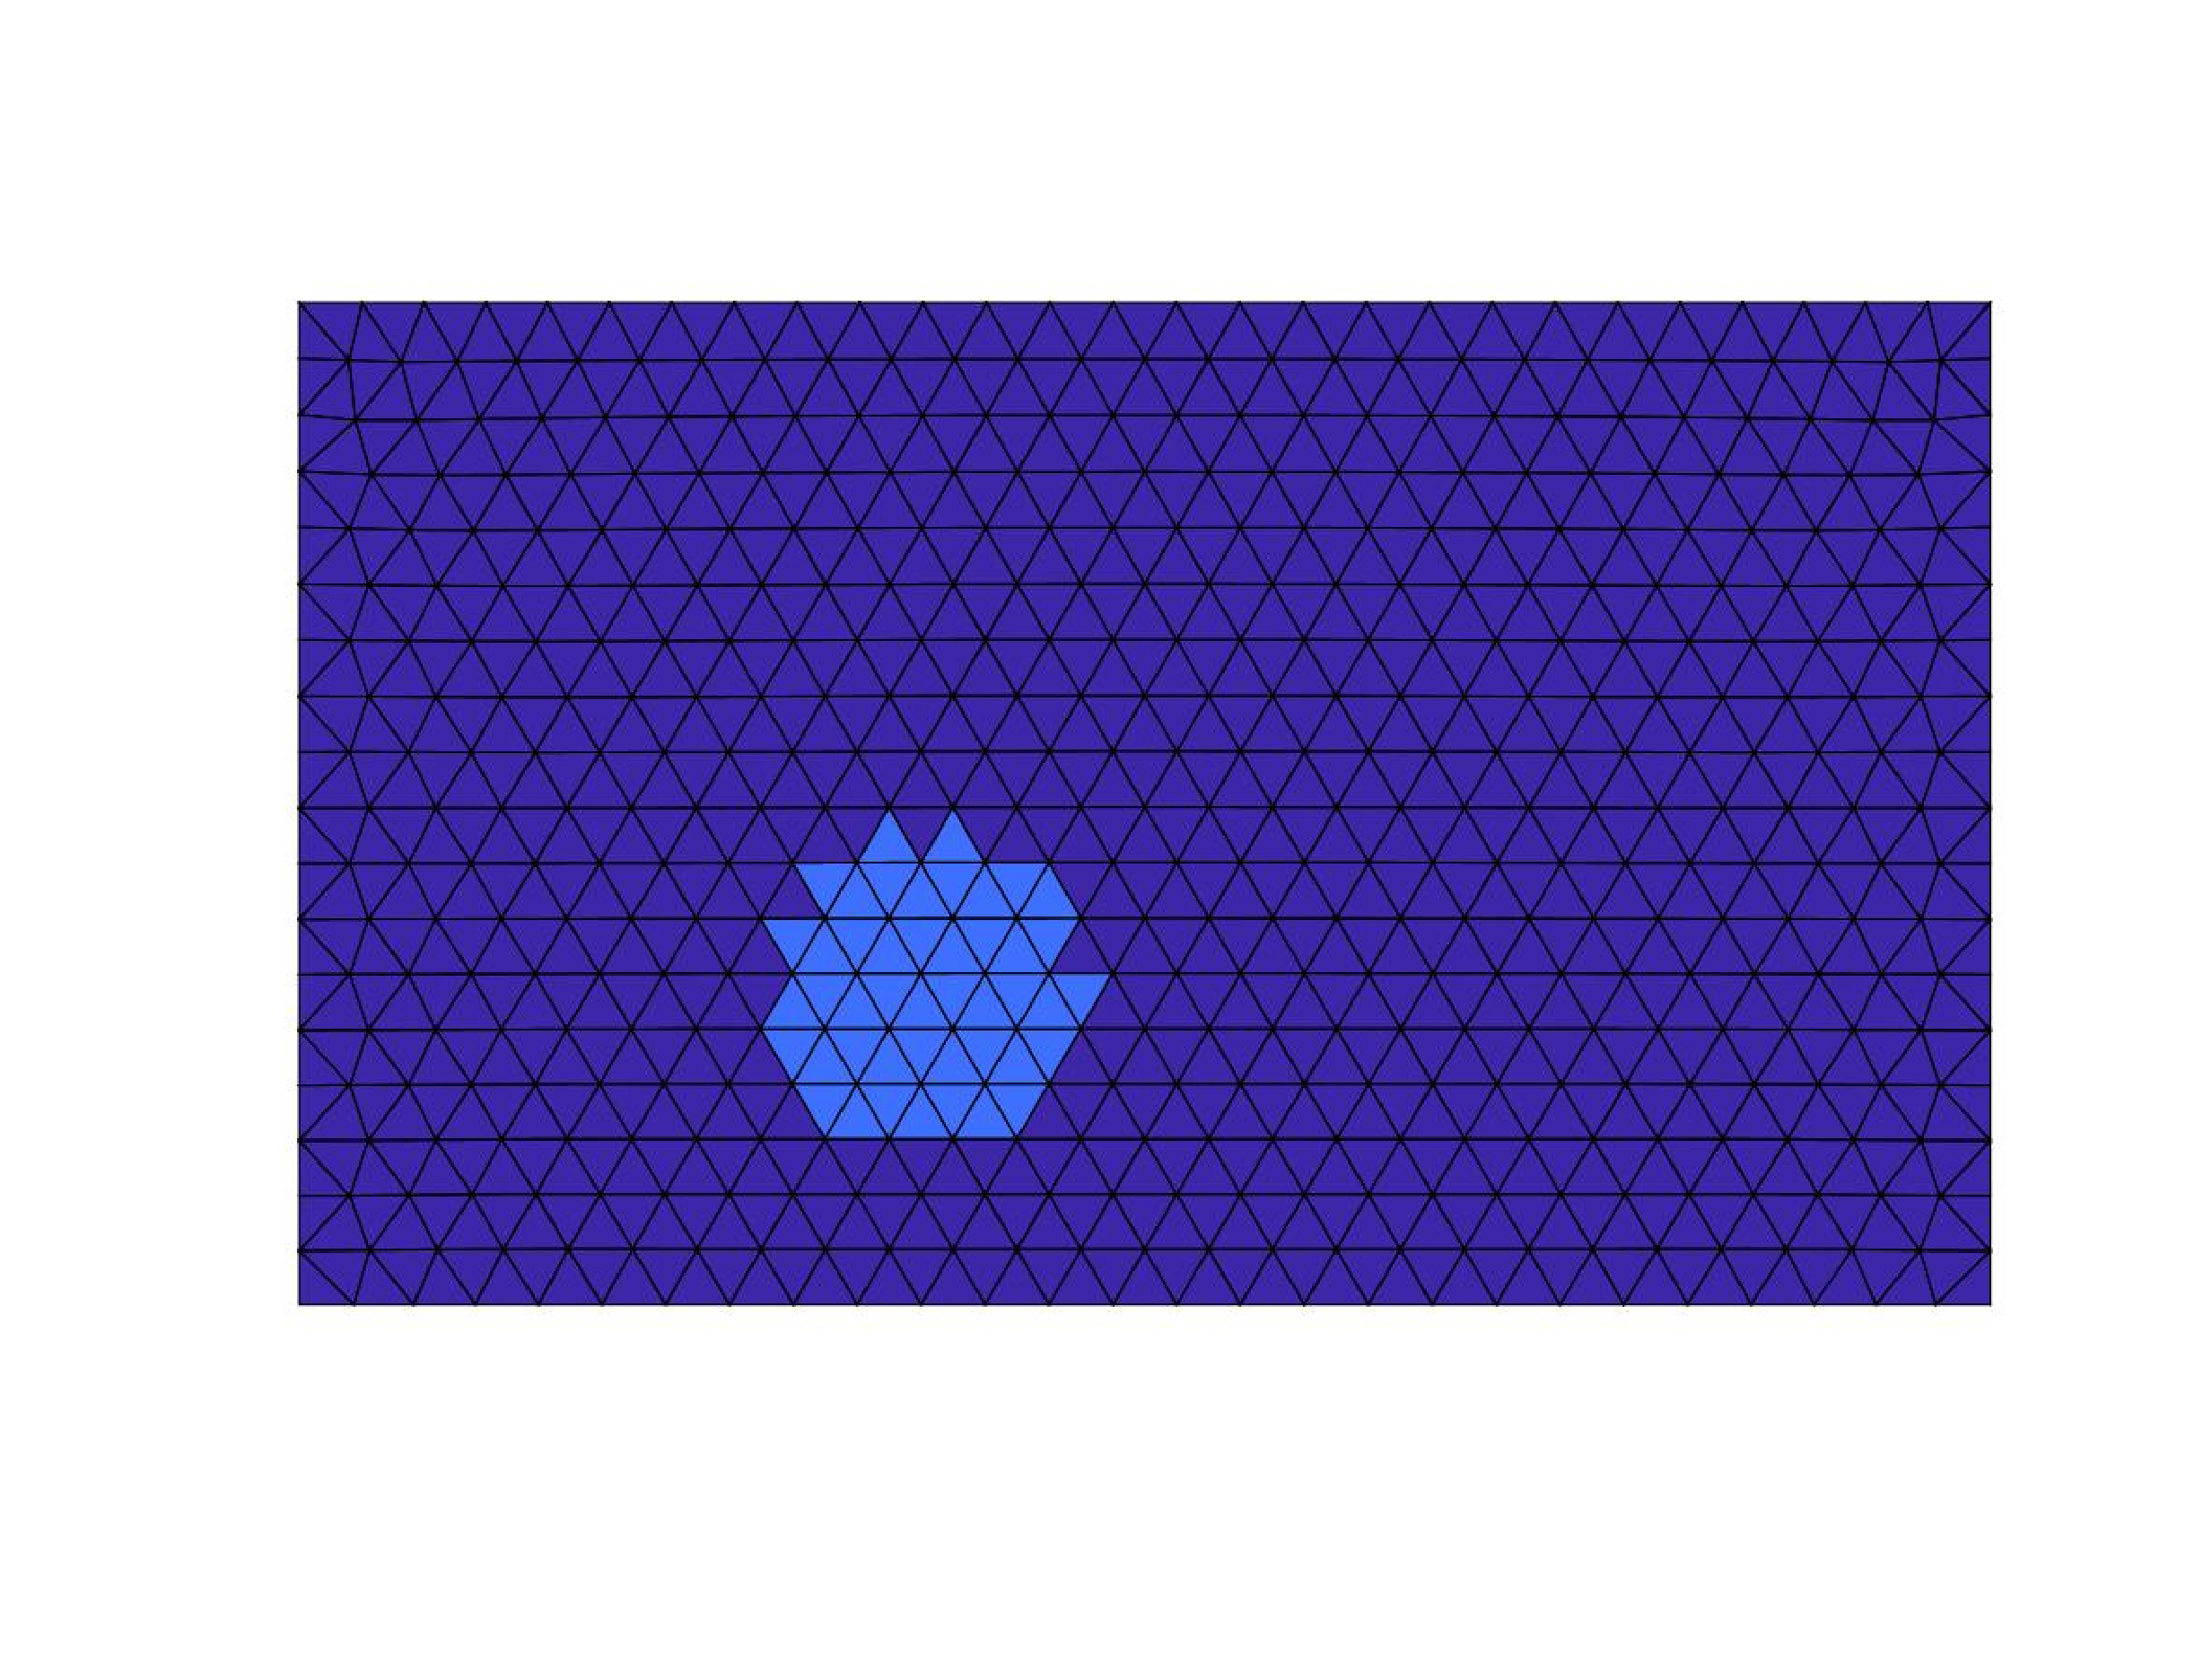
\includegraphics[trim = 0mm 40mm 80mm 40mm, clip=true,width=0.8\linewidth]{img/ruptuerprocess_step1.eps}
    \caption{ 平面断层模型(图中浅色区为初始破裂)} \label{fig:rupture-model1}
  \end{figure}
    \noindent 一共有~958~个单元,525~个点。初始的破裂区为以网格坐标(0.25,1)为中心,半径为0.25公里的圆形区域~(如图~\ref{fig:rupture-model1}~中浅色区所示)。P~波数波速为~5.6km/s~,S波波速为~3.23km/s。断层的初始应力分布为:圆形区域的初始应力大于破裂强度,大小为~$\sigma_{0} = 1.2 T_0$,圆形以外的区域初始应力小于破裂强度,大小为~$\sigma_{0}=0.8T_{0}$~。 在该初始应力条件下,该平面断层为以中间圆为初始破裂区域进行自发破裂过程。一共计算~150~个时间步。我们分别采用两种方法来计算积分核值。可以得到,用原有方法计算积分核需要~936.98s。 而我们采用分区处理的办法,计算积分核 只需要~269.5s,效率提高了~71.2\%。最后,将由分区法所得的积分核用以破裂过程的计算,可以得到破裂图像如图~\ref{fig:rupture-process}~所示。可见,在保证正确性的条件下,分区计算积分核 的方法具有更高的效率。
    
\begin{figure}[!h]
  \centerin
  \includegraphics[width=0.99\linewidth]{img/rupture1.png}
    \caption{ 平面断层破裂过程} \label{fig:rupture-process}
 \end{figure}
  
    \begin{comment}
    \begin{figure}[!h]
  \centering
  \begin{subfigure}[b]{0.3\linewidth}
    \includegraphics[trim = 20mm 30mm 20mm 30mm,clip=true,width=\linewidth]{img/ruptuerprocess_step3.jpg}
    %\label{a}
  \end{subfigure}
  \begin{subfigure}[b]{0.3\linewidth}
    \includegraphics[trim = 20mm 30mm 20mm 30mm,clip=true,width=\linewidth]{img/ruptuerprocess_step10.jpg}
  \end{subfigure}
  \begin{subfigure}[b]{0.3\linewidth}
    \includegraphics[trim = 20mm 30mm 20mm 30mm,clip=true,width=\linewidth]{img/ruptuerprocess_step20.jpg}
  \end{subfigure}
  \begin{subfigure}[b]{0.3\linewidth}
    \includegraphics[trim = 20mm 30mm 20mm 30mm,clip=true,width=\linewidth]{img/ruptuerprocess_step30.jpg}
  \end{subfigure}
  \begin{subfigure}[b]{0.3\linewidth}
    \includegraphics[trim = 20mm 30mm 20mm 30mm,clip=true,width=\linewidth]{img/ruptuerprocess_step35.jpg}
    %\label{a}
  \end{subfigure}
  \begin{subfigure}[b]{0.3\linewidth}
    \includegraphics[trim = 20mm 30mm 20mm 30mm,clip=true,width=\linewidth]{img/ruptuerprocess_step40.jpg}
  \end{subfigure}
  \begin{subfigure}[b]{0.3\linewidth}
    \includegraphics[trim = 20mm 30mm 20mm 30mm,clip=true,width=\linewidth]{img/ruptuerprocess_step50.jpg}

  \end{subfigure}
  \begin{subfigure}[b]{0.3\linewidth}
    \includegraphics[trim = 20mm 30mm 20mm 30mm,clip=true,width=\linewidth]{img/ruptuerprocess_step55.jpg}
  \end{subfigure}
  \begin{subfigure}[b]{0.3\linewidth}
    \includegraphics[trim = 20mm 30mm 20mm 30mm,clip=true,width=\linewidth]{img/ruptuerprocess_step60.jpg}
    %\label{a}
  \end{subfigure}
  \begin{subfigure}[b]{0.3\linewidth}
    \includegraphics[trim = 20mm 30mm 20mm 30mm,clip=true,width=\linewidth]{img/ruptuerprocess_step70.jpg}
  \end{subfigure}
  \begin{subfigure}[b]{0.3\linewidth}
    \includegraphics[trim = 20mm 30mm 20mm 30mm,clip=true,width=\linewidth]{img/ruptuerprocess_step80.jpg}
  \end{subfigure}
  \begin{subfigure}[b]{0.3\linewidth}
    \includegraphics[trim = 20mm 30mm 20mm 30mm,clip=true,width=\linewidth]{img/ruptuerprocess_step90.jpg}
  \end{subfigure}
  \caption{ 平面断层破裂过程66}
\end{figure}
\end{comment}
   
		\subsection{数值算例二}
    \indent 接着我们考虑一个复杂断层系统的情况。研究的断层为一弯折断层,如图~\ref{fig:rupture-model2}~所示。该弯折断层由三个平面构成,其中弯折的平面与水平面夹角为~$40.13^{\circ}$。该弯折断层离散为1073个单元,624个点。在弯折断层的第一个平面设置与数值算例一中平面断层上相同的圆形破裂区。
    
    \begin{figure}[H]
 \centerin
  \includegraphics[width=0.8\linewidth]{img/3Druptuerprocess_step1.png}
    \caption{ 弯折断层模型(图中浅色区为初始破裂区)} \label{fig:rupture-model2}
  \end{figure}
 \indent 一共计算~200~个时间步。同样的我们仍然采用两种计算方式计算积分核的值。若采用原方法需要~2298.41s才能计算得出结果,而采用分区计算积分核的方式,计算时长为~663.0s。计算效率提高了~71.14\%。利用计算所得的积分核可以得到破裂过程图如图~\ref{fig:3d-rupture}~所示。
 
 \begin{figure}[!h]
  \centerin
  \includegraphics[width=0.99\linewidth]{img/rupture2.png}
    \caption{ 弯折断层破裂过程} \label{fig:3d-rupture}
 \end{figure}
 
   \begin{comment}
    \begin{figure}[!h]
  \centering
    \begin{subfigure}[b]{0.45\linewidth}
    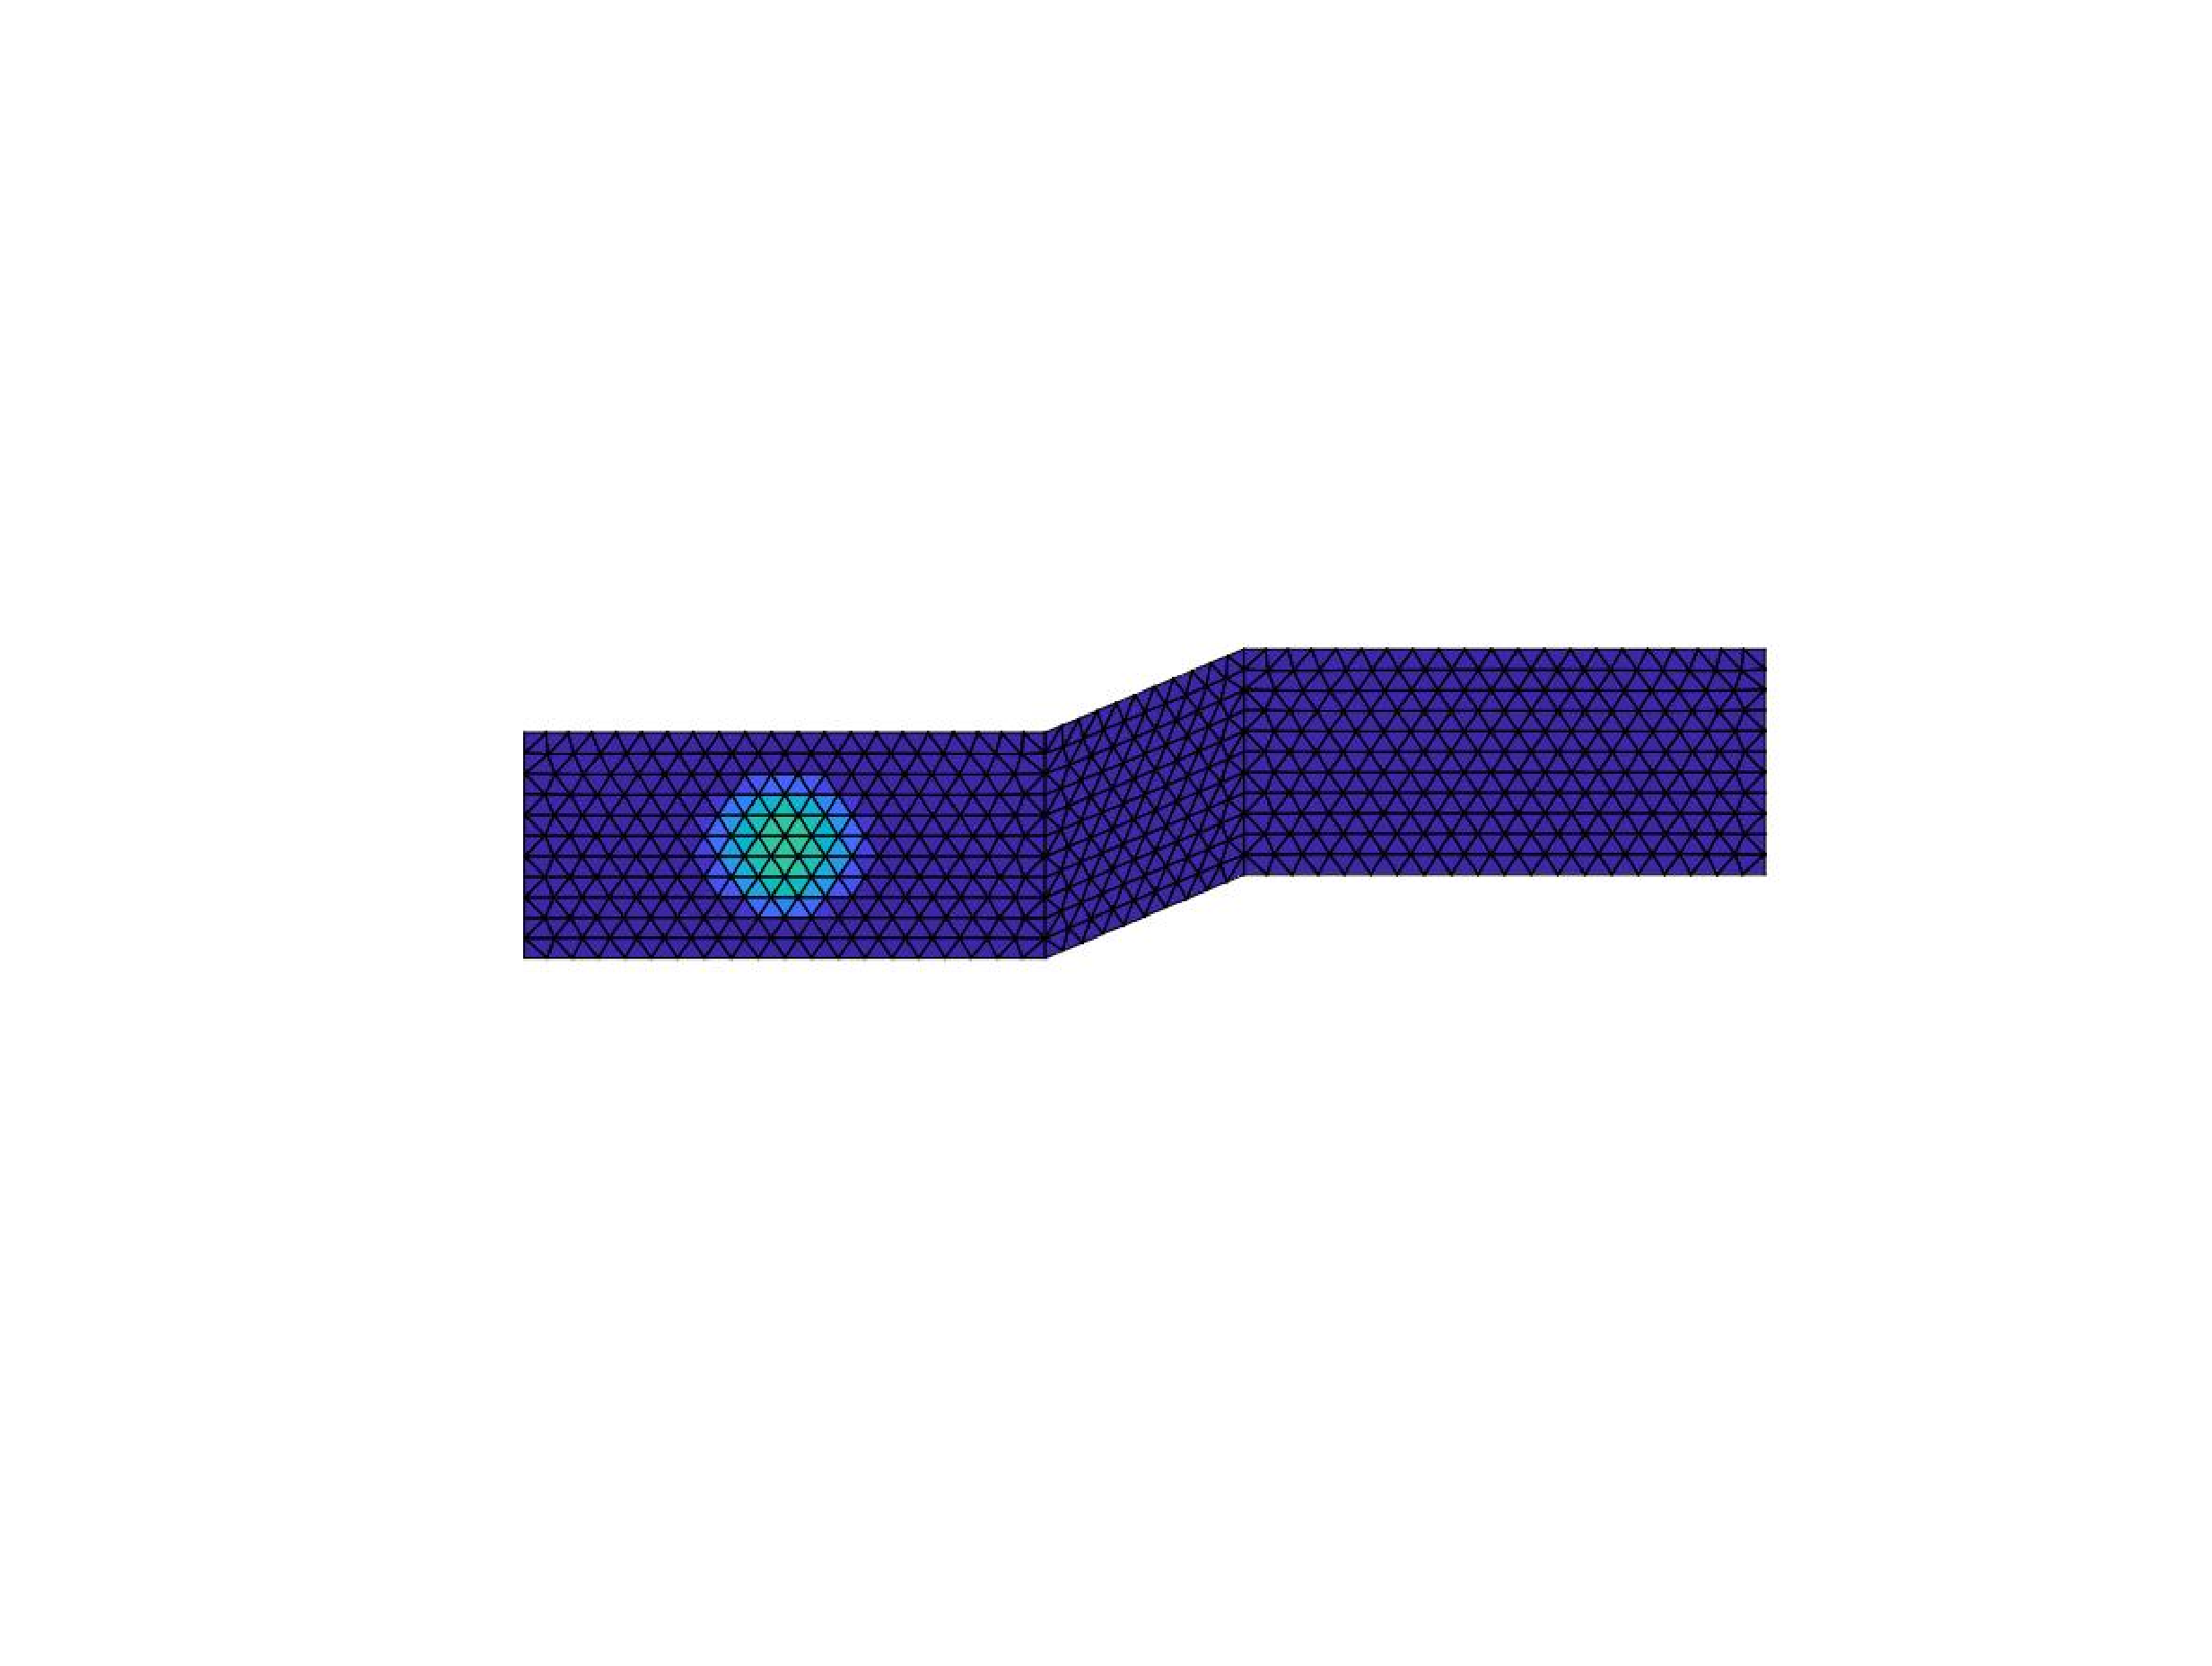
\includegraphics[trim = 100mm 120mm 100mm 120mm,clip=true, width=\linewidth]{img/3Druptuerprocess_step10.eps}
  \end{subfigure}
    \begin{subfigure}[b]{0.45\linewidth}
    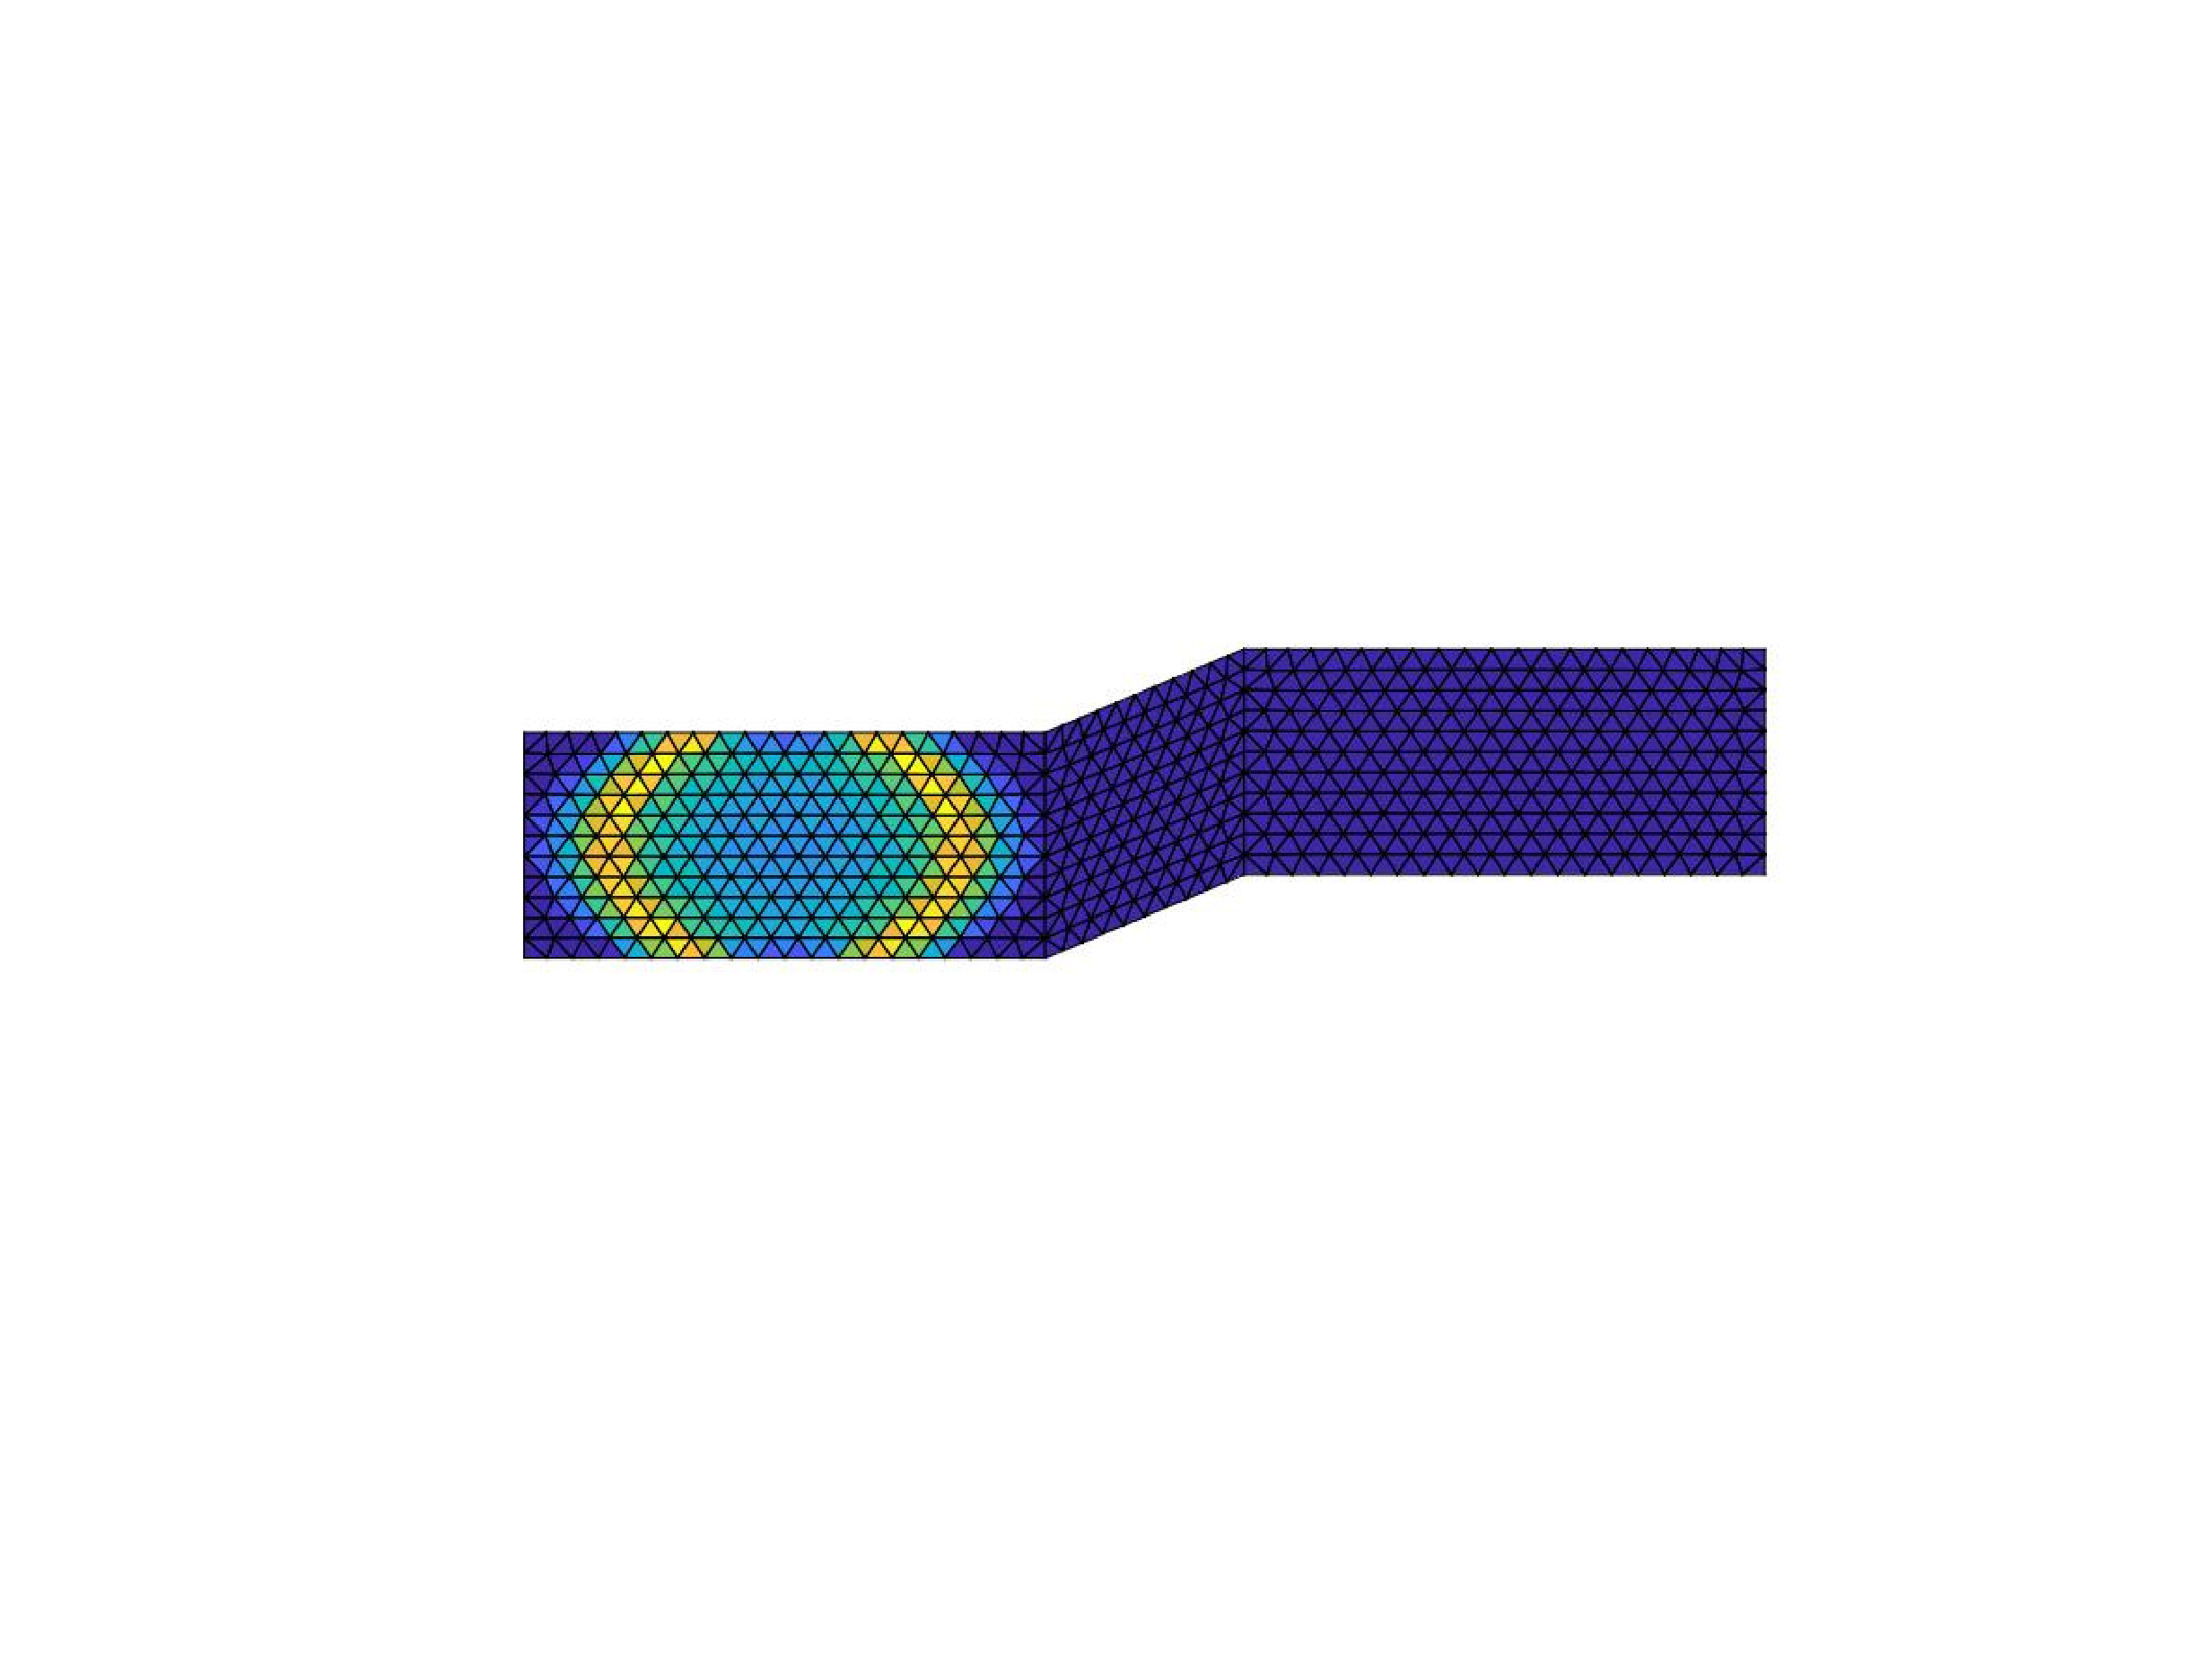
\includegraphics[trim = 100mm 120mm 100mm 120mm,clip=true, width=\linewidth]{img/3Druptuerprocess_step60.eps}
  \end{subfigure}
  
  \begin{subfigure}[b]{0.45\linewidth}
    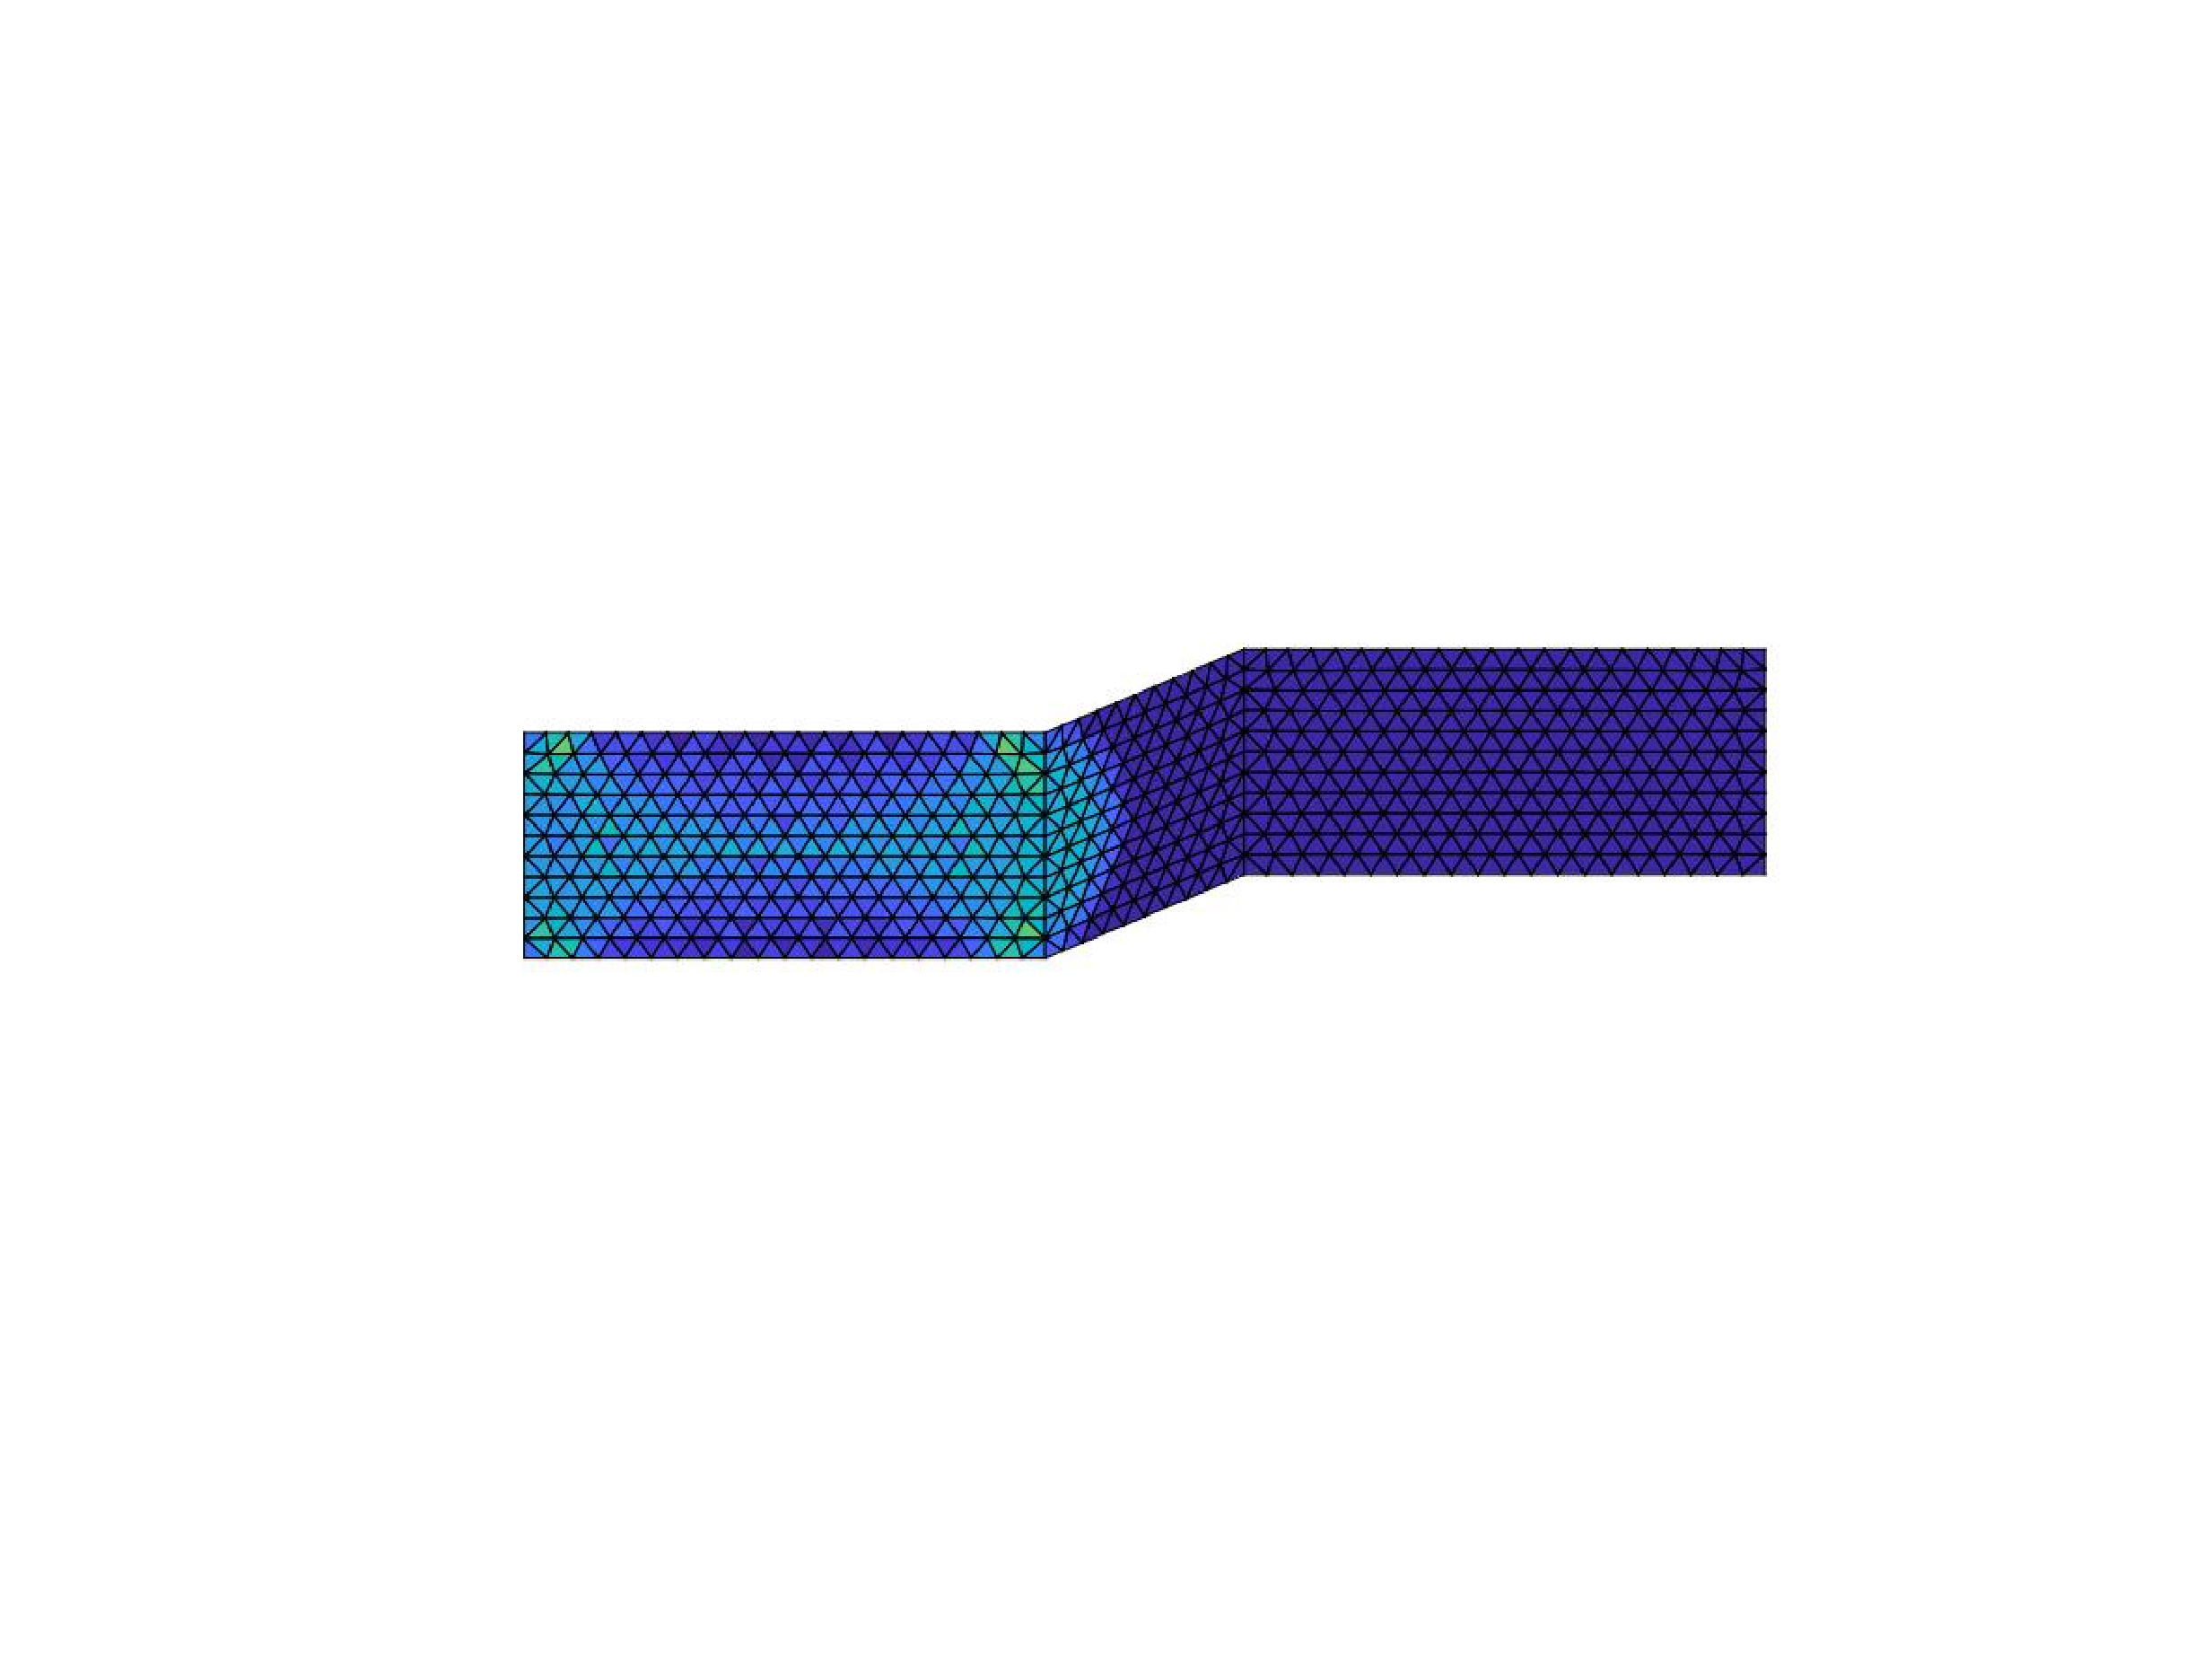
\includegraphics[trim = 100mm 120mm 100mm 120mm,clip=true, width=\linewidth]{img/3Druptuerprocess_step90.eps}
  \end{subfigure}
  \begin{subfigure}[b]{0.45\linewidth}
    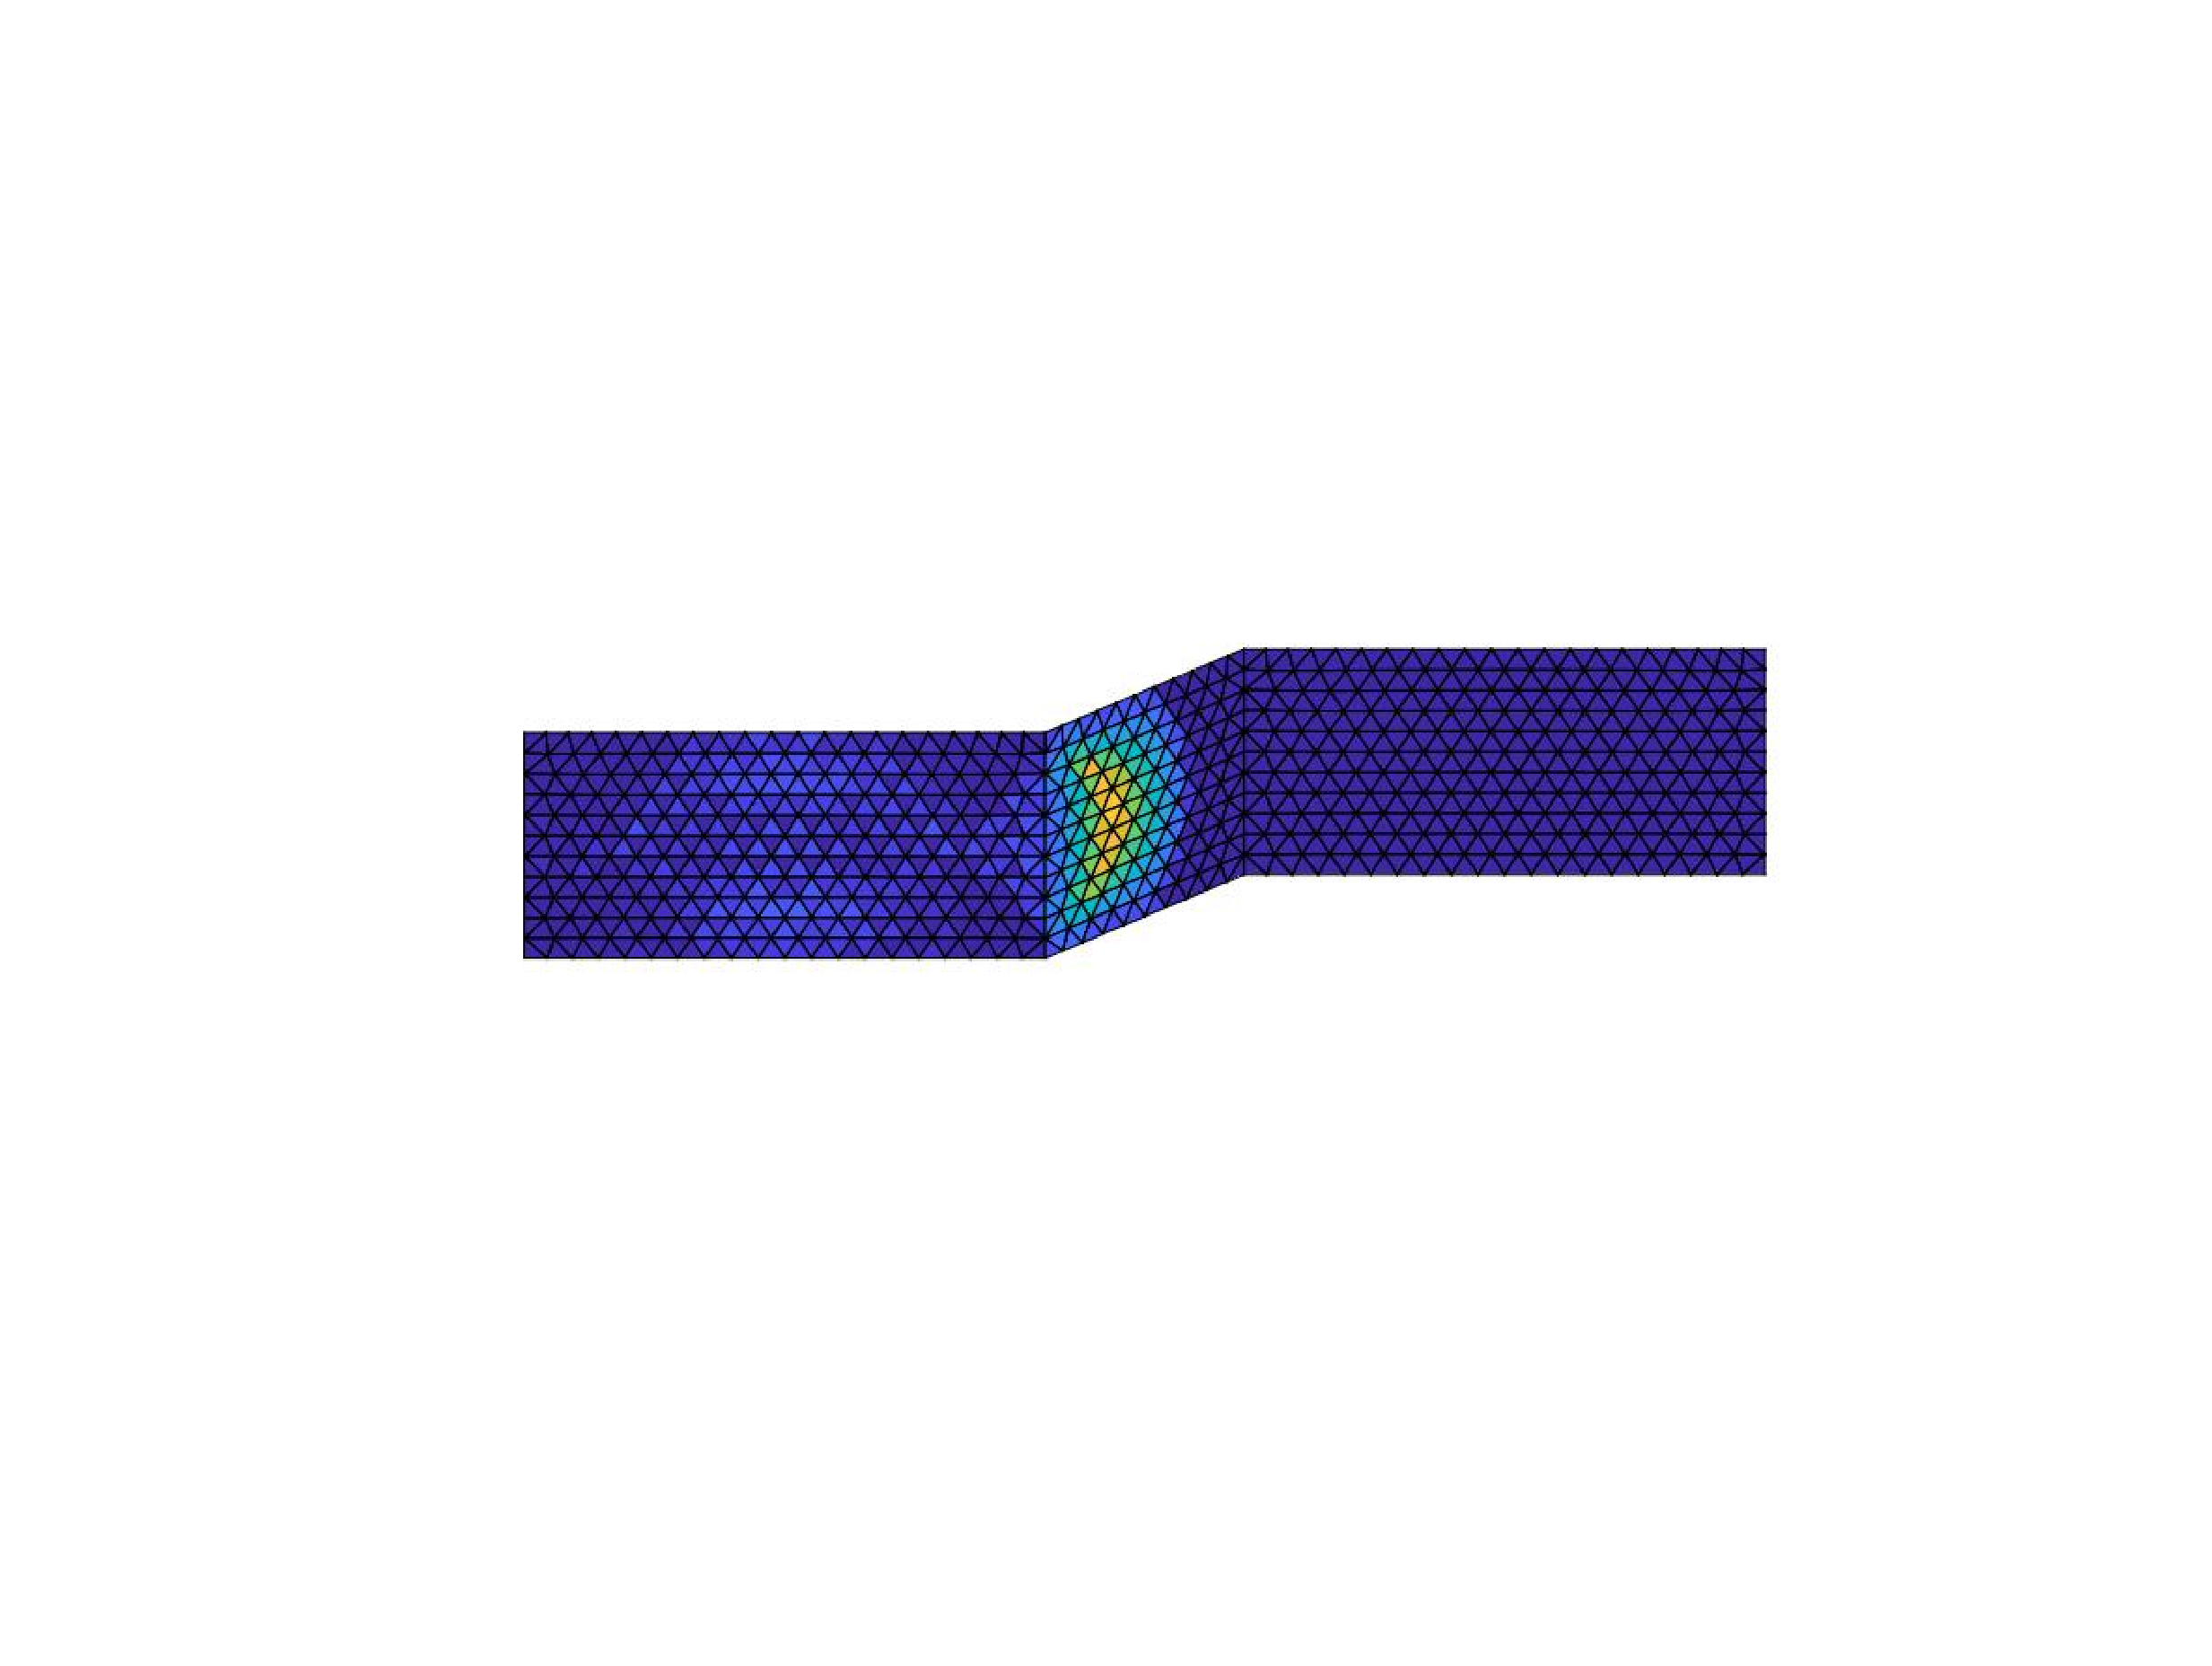
\includegraphics[trim = 100mm 120mm 100mm 120mm,clip=true, width=\linewidth]{img/3Druptuerprocess_step110.eps}
  \end{subfigure}
  
  \begin{subfigure}[b]{0.45\linewidth}
    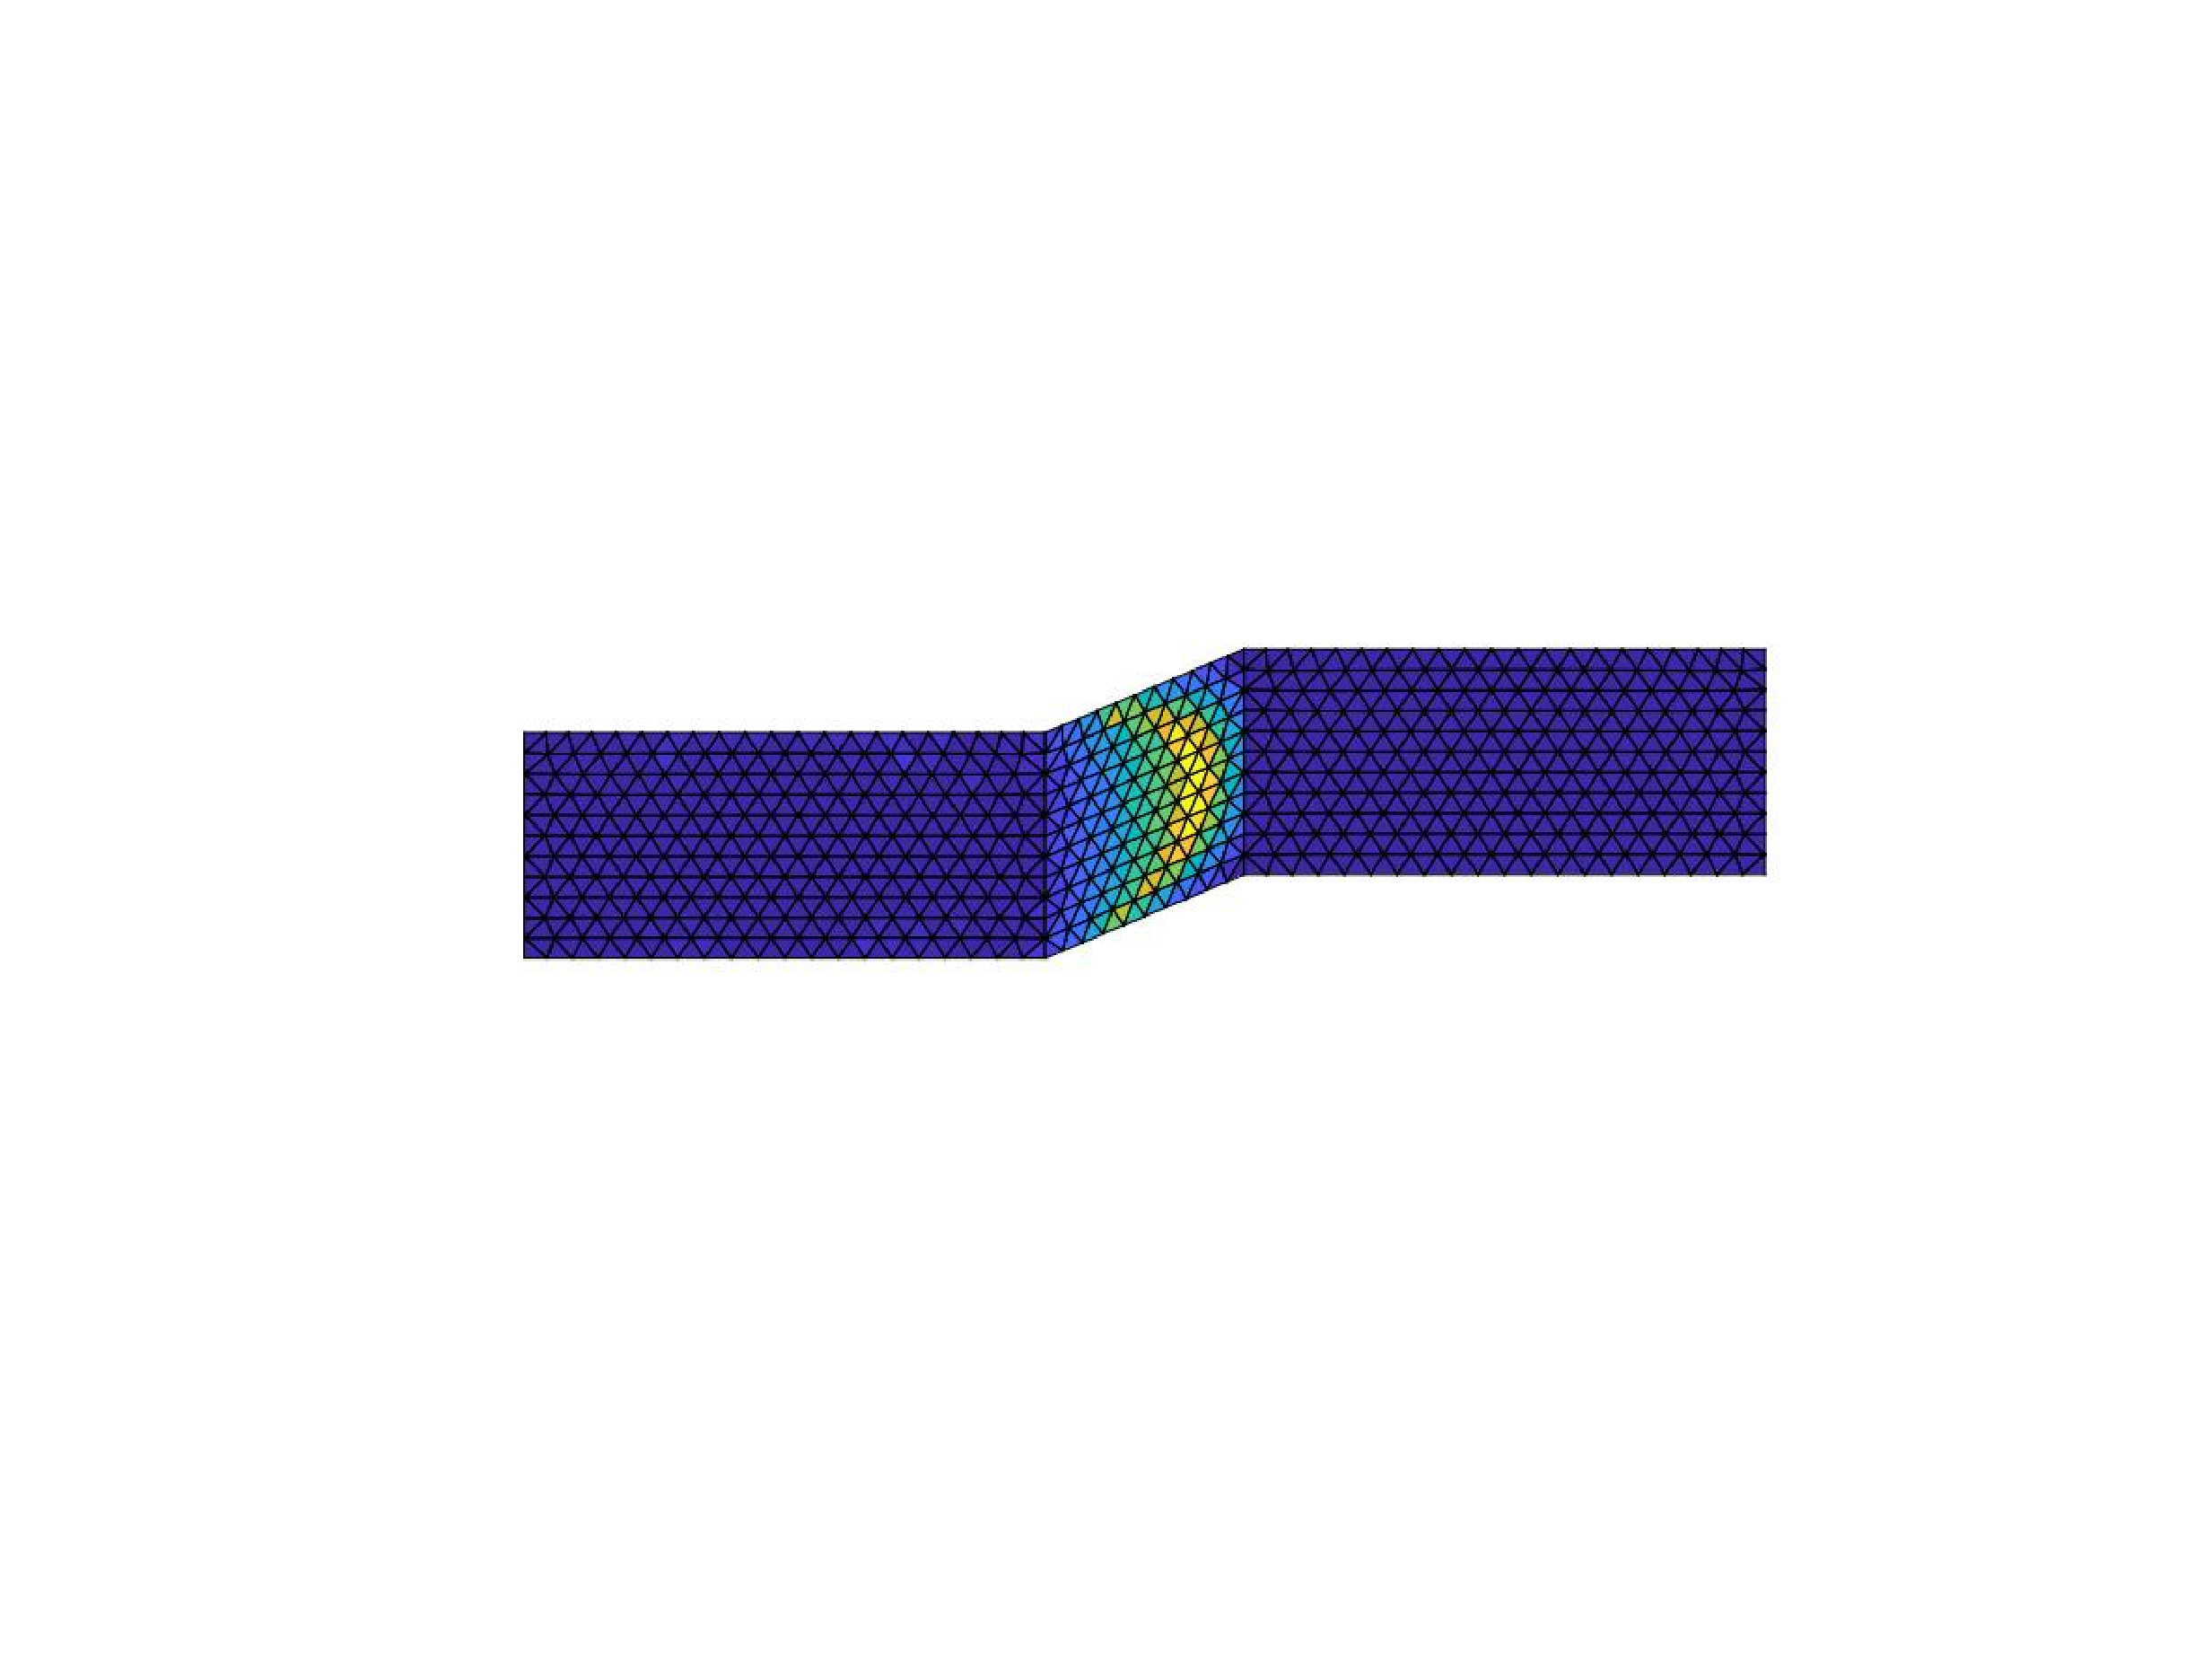
\includegraphics[trim = 100mm 120mm 100mm 120mm,clip=true, width=\linewidth]{img/3Druptuerprocess_step130.eps}
  \end{subfigure}
  \begin{subfigure}[b]{0.45\linewidth}
    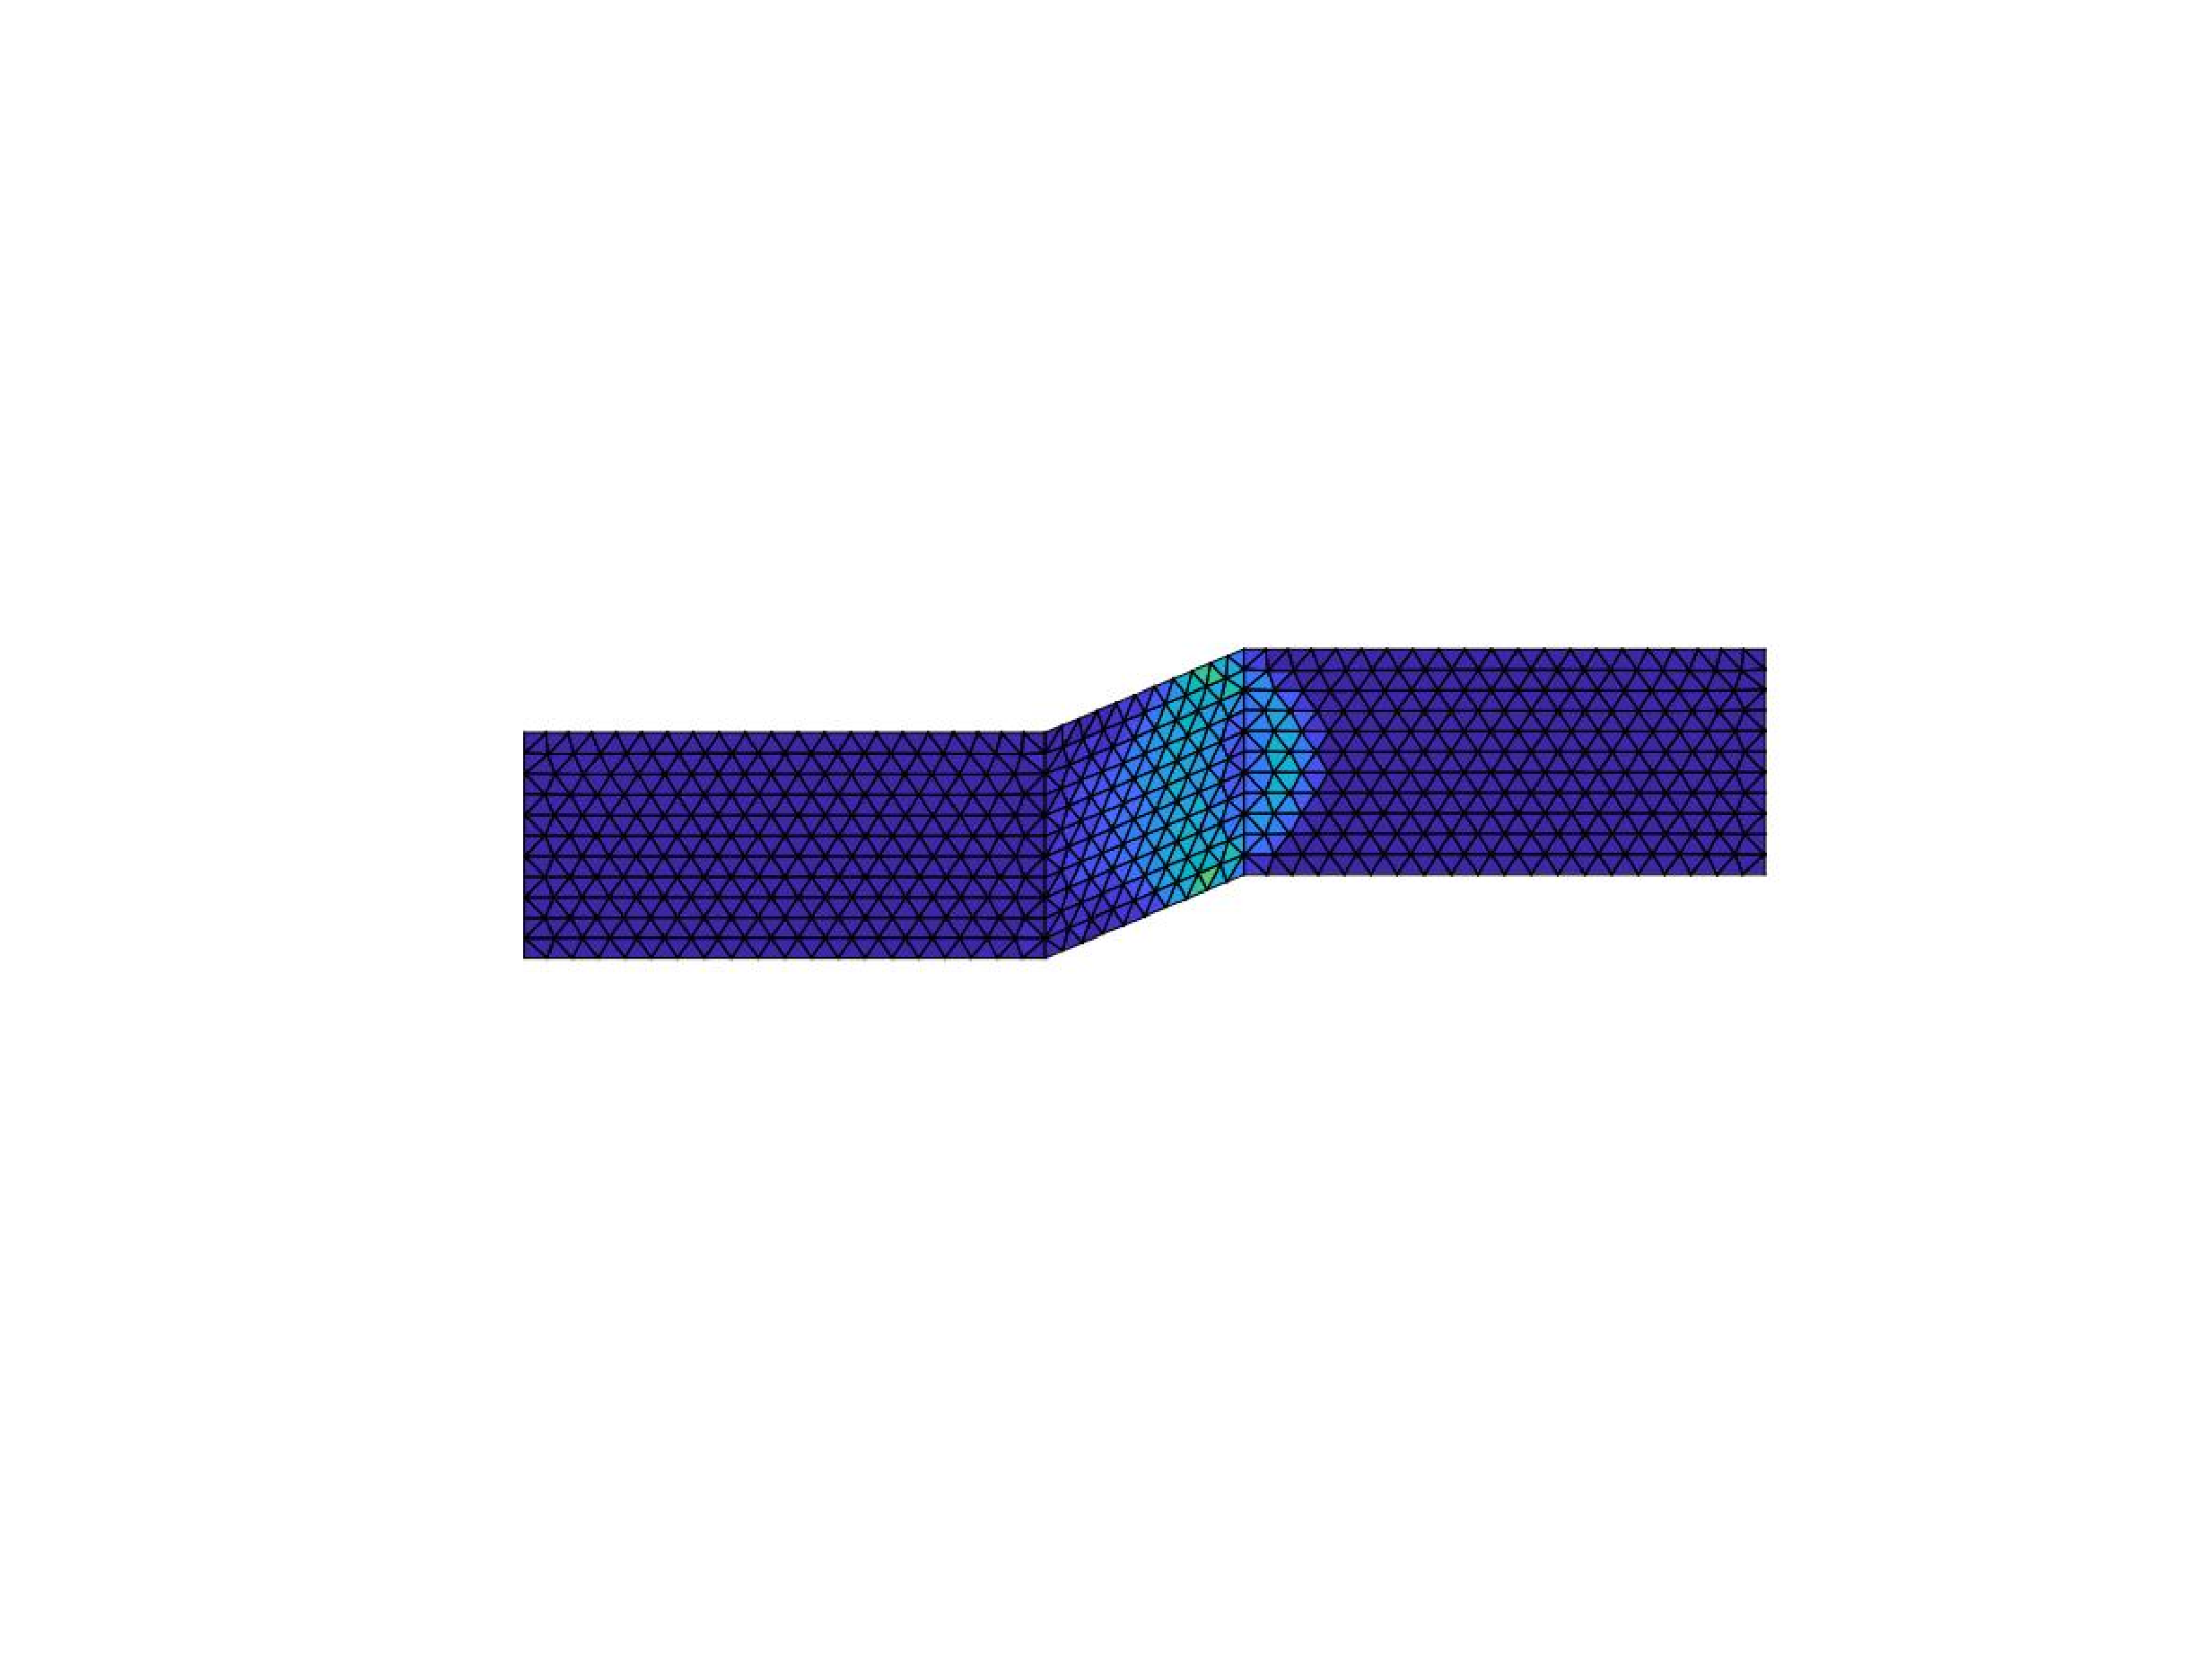
\includegraphics[trim = 100mm 120mm 100mm 120mm,clip=true, width=\linewidth]{img/3Druptuerprocess_step150.eps}
  \end{subfigure}
  \begin{subfigure}[b]{0.45\linewidth}
    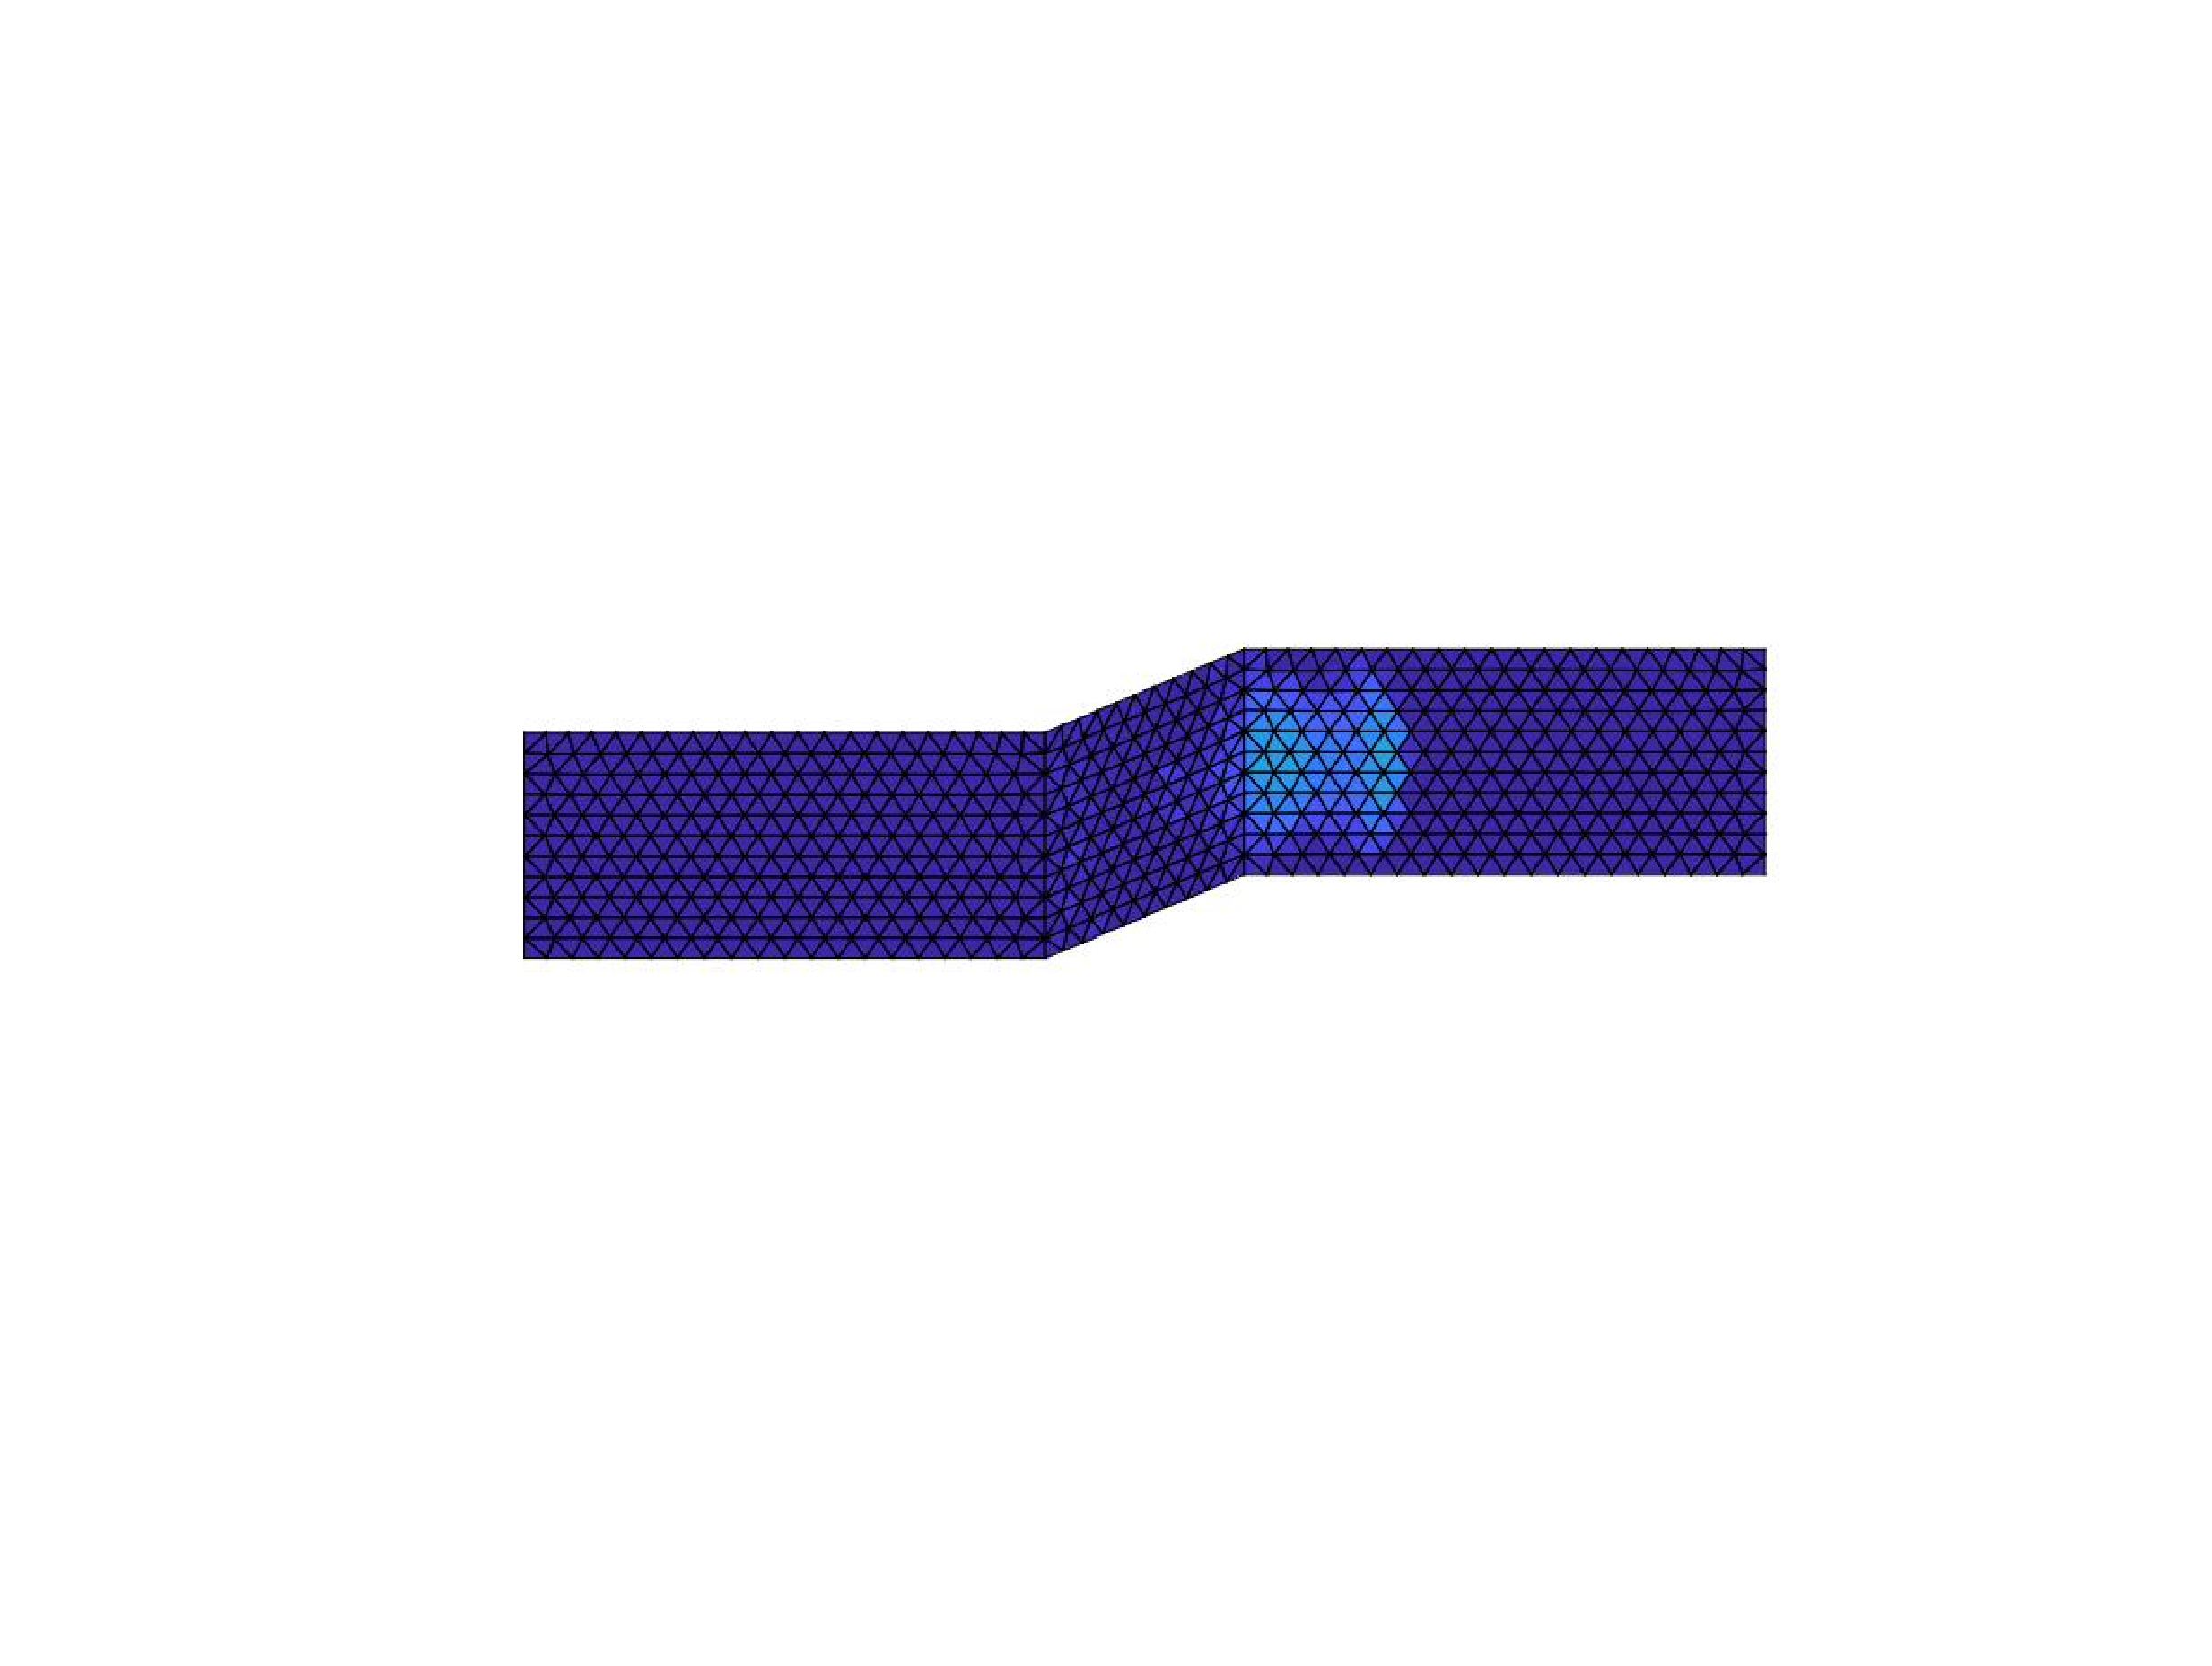
\includegraphics[trim = 100mm 120mm 100mm 120mm,clip=true, width=\linewidth]{img/3Druptuerprocess_step170.eps}
  \end{subfigure}
  \begin{subfigure}[b]{0.45\linewidth}
    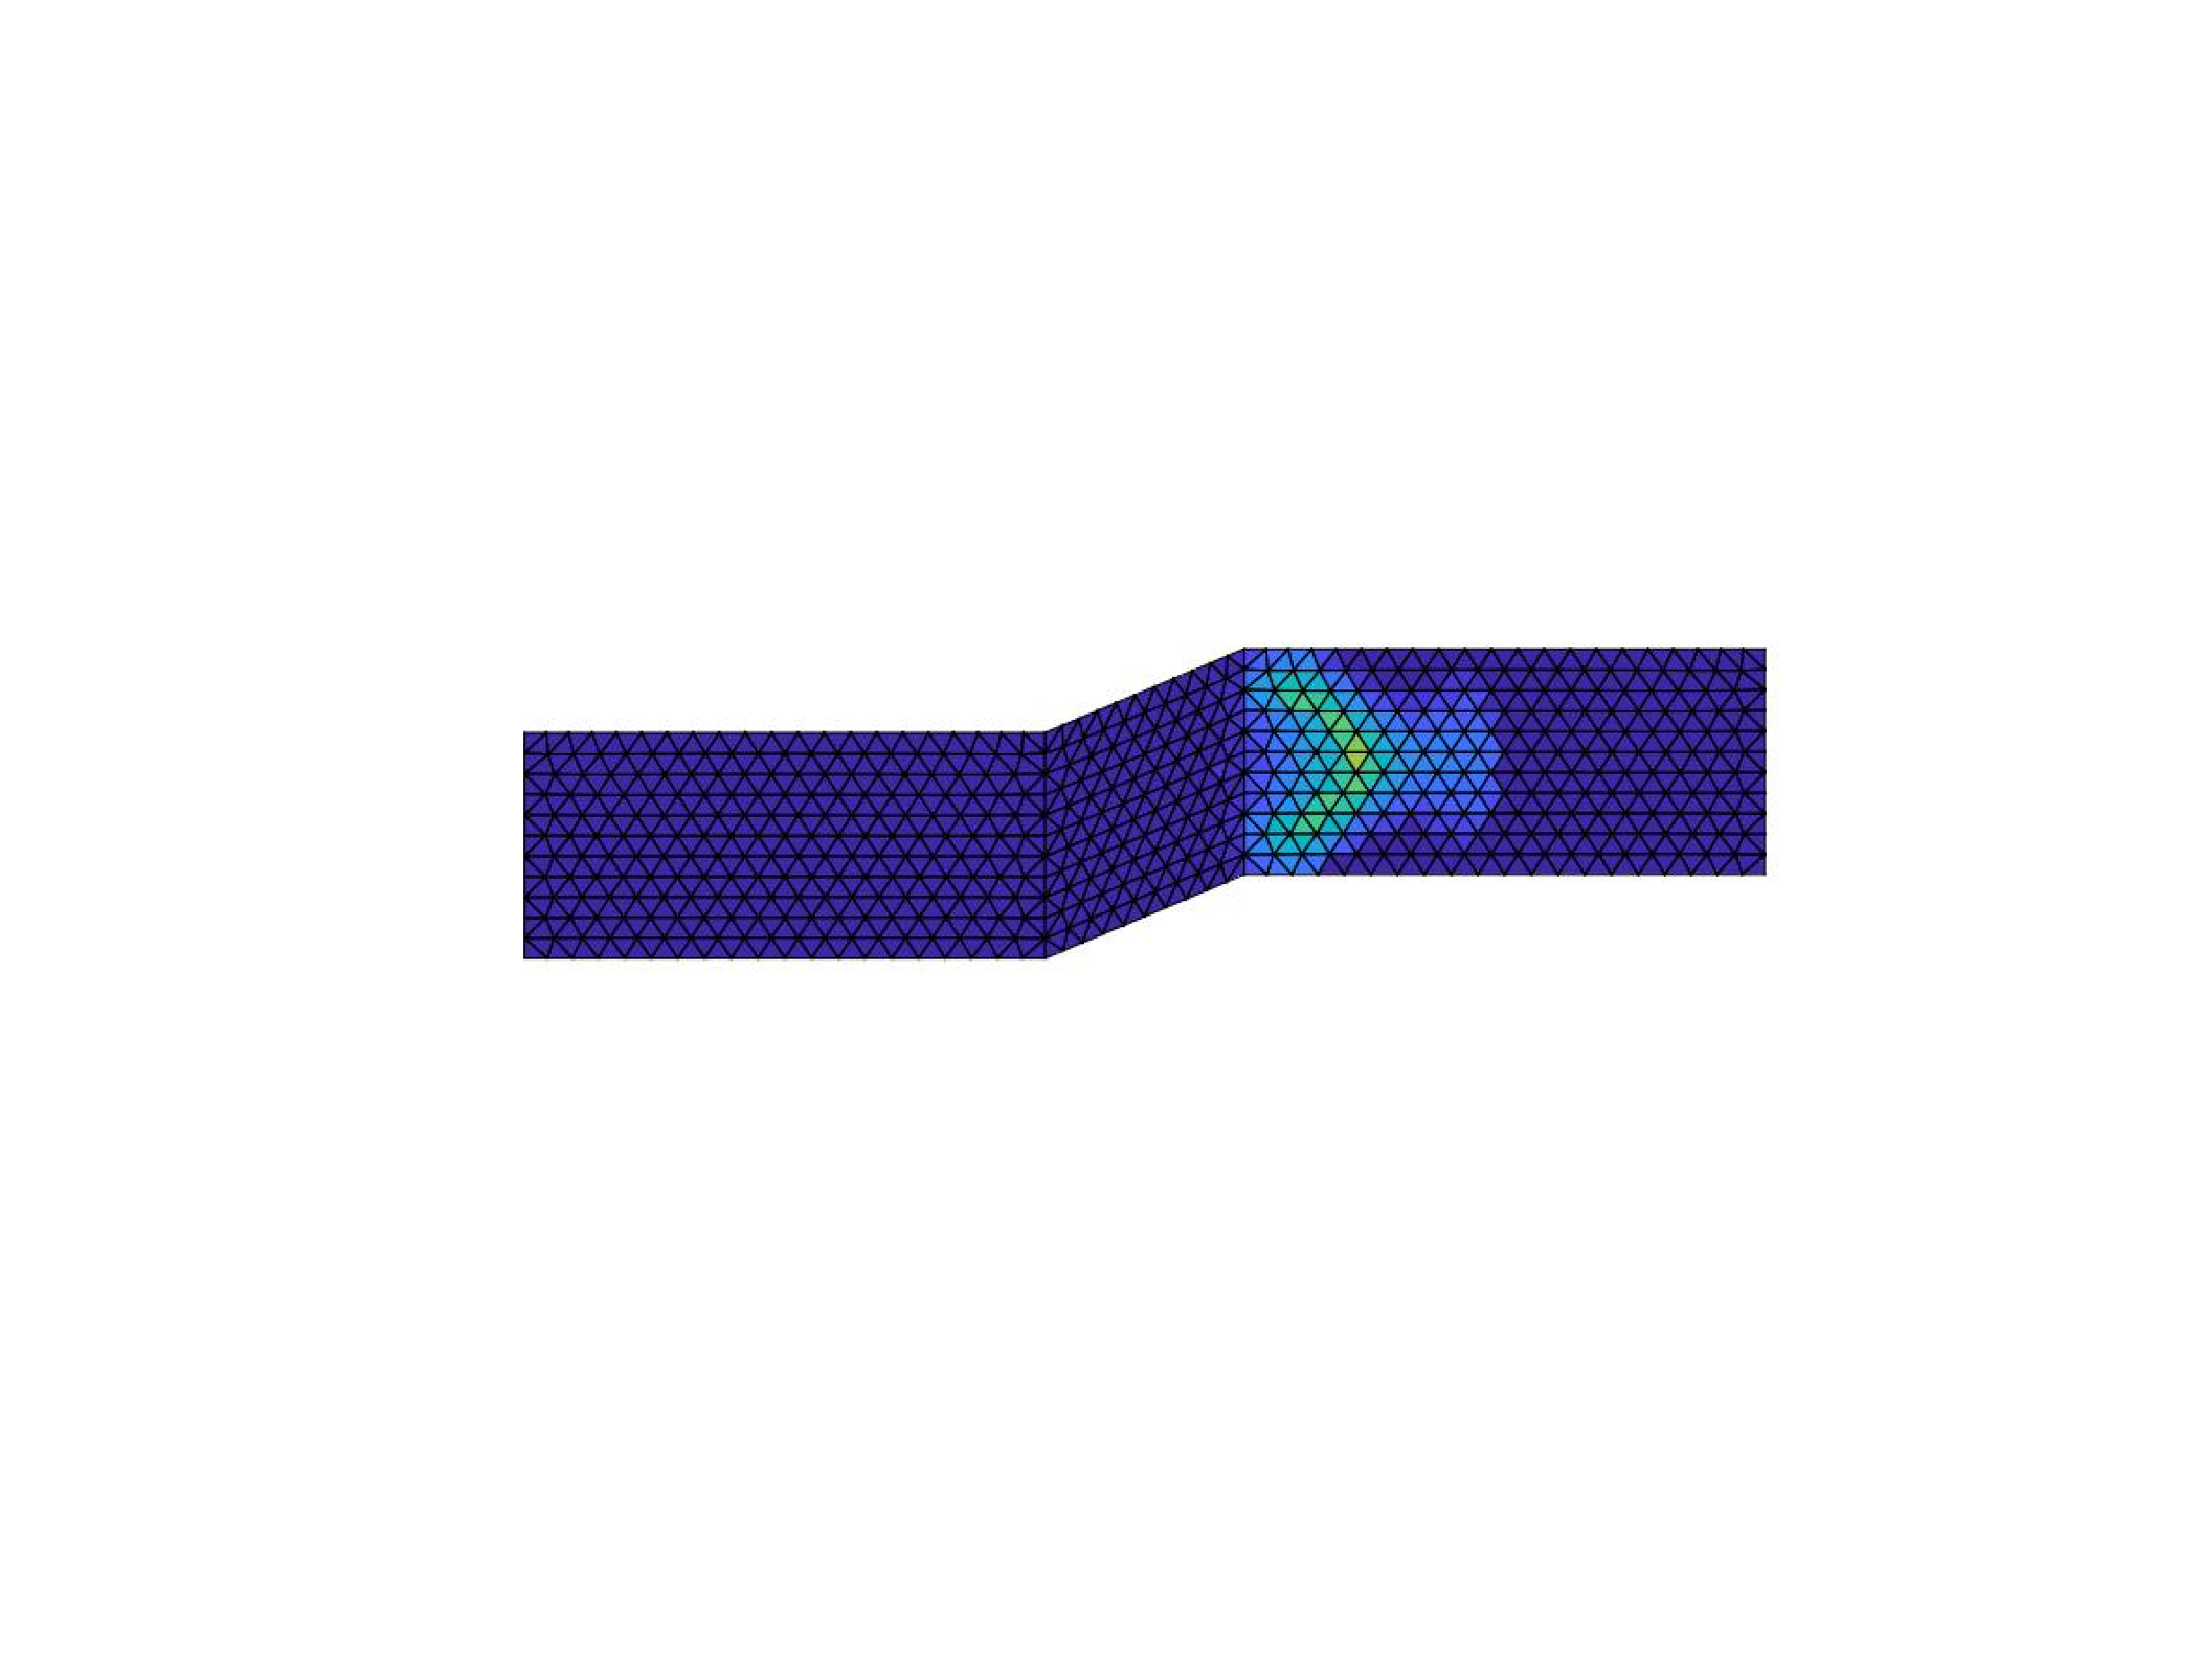
\includegraphics[trim = 100mm 120mm 100mm 120mm,clip=true, width=\linewidth]{img/3Druptuerprocess_step190.eps}
  \end{subfigure}
    \caption{ 弯折断层破裂过程}\label{fig:3d-rupture}
\end{figure}
\end{comment}
	\section{结论分析}
	\indent 在原方法中,积分核计算的时间复杂度为~$O(M^{3}N)$。其中~M~为单元数,N~为时间步。在实际的破裂模拟中,存在许多大尺度即单元数目非常多的模型,若不采取任何加速计算方案将会产生巨大的时间开销。而采用分区计算的加速方案,能够节省~70\%~以上的时间,将大大提高断层破裂过程模拟的效率。

\chapter{总结与展望}
\indent 本文期望实现的目标最终得到了一个不错的结果,即通过分区处理的办法,使得数值模拟破裂过程中积分核值的计算效率得到了显著的提高。我们从~Feng and Zhang(2017)~推导的计算积分核的公式出发,通过到时的不同划分了三个不同区域:初始区,传播区,稳定区。而在初始区和稳定区中,积分核的计算公式得到了相应的简化。通过简化后的表达式我们能快速确定在初始区和稳定区对应的积分核,从而达到了提高计算效率的目的。从本文的分析可以看出,初始区和稳定区的计算占据了积分核计算的绝大部分计算成本。因此对于这两个区域进行加速处理也是很有必要的。一方面我们能以更高的速率获得结果,另一方面可以节约计算资源。而在最后,通过数值算例的验证,既检验了分区计算积分核方法的正确性,另一方面也从实际算例体现了分区法在计算速率上的优越性。\\
\indent 本文虽然对破裂过程中积分核的计算进行极大的优化,但是从分区计算的物理过程我们可以知道,积分核的大部分为0或者稳定值,即在数学上,我们获得的积分核 值为一个三维的稀疏矩阵。而我们在破裂过程的计算中使用了整个矩阵,以为着有大量的0或者稳定值被存入了内存中,造成了内存使用的浪费。因此有必要对于参与破裂过程的积分核矩阵进行一定的压缩处理,以提高内存的利用率。这一部分工作已经展开,详细结果将在附录A中展示。已经实现的情况是,能够对矩阵中所有的~0~元素进行压缩处理。然而又有新的问题产生,为了提高内存的使用率,目前的测量增加了计算的时间的复杂度,也即拿时间换空间。这样的矩阵压缩处理导致了计算效率的降低,与我们最初提升整程序计算效率的初衷相违背。因此,在未来的工作中,如何在增加更小时间复杂的情况下实现对于矩阵的充分压缩是一个需要进一步研究的问题。\\
\indent 无论是对于积分核分区处理达到加速的目的,还是在破裂计算的过程中,压缩矩阵以减小内存的使用,本文的工作都是震源动力学很小的一个方面。但是随着研究的进展,逐渐了解了相关的一些知识,比如网格化分,复杂断层研究等。目前的工作,将为我们进一步学习和研究震源动力学提供一个一窥其究的窗口。






	\chapter{机器学习方法预估震级效果评估与讨论 }
\section{数据分析与预处理}
\indent 利用第二、三章所描述的方法,本文搭建并实现了$\tau_{c}$方法和机器学习类模型进行效果检验。考虑到震级紧急预估的应用场景和所需要的基础设施需求,我们将研究区域定位日本岛区域。原始全数据集使用了日本KIK和KNET两台站网从2015至2017年所记录到的所有大于3级且震源靠近日本岛主体的地震记录,除此之外并无经过其他任何的主动事件挑选,事件分布如下图4.1所示。\\
\begin{figure}[!h] 
\centering 
 \includegraphics[width=0.8\linewidth]{img/basemap.jpg} 
 \renewcommand{\figurename}{图} 
\caption{全数据集地震事件} 
%英文标题begin 
\addtocounter{figure}{-1} \vspace{-5pt} 
%\SetEnglishCaption 
\renewcommand{\figurename}{Fig} 
\caption{Full data set earthquake event} 
\renewcommand{\figurename}{图} 
%英文标题end 
\label{fig:network-device-influence.png} 
\end{figure}
\indent 原始全数据中共包含了840个地震事件,合计50314条记录,具体的分布和统计如下图4.2和4.3所示,其中包含了3级至4级地震事件共420个、10145条地震台站记录,4级至5级地震事件共216个、14629条地震台站记录,5级至6级地震事件共61个、10740条地震台站记录,6级以上地震事件共8个、1004条地震台站记录。\\
\begin{figure}[!h] 
\centering 
 \includegraphics[width=0.95\linewidth]{img/Event distribution.png} 
 \renewcommand{\figurename}{图} 
\caption{全数据集地震事件} 
%英文标题begin 
\addtocounter{figure}{-1} \vspace{-5pt} 
%\SetEnglishCaption 
\renewcommand{\figurename}{Fig} 
\caption{Full data set earthquake event} 
\renewcommand{\figurename}{图} 
%英文标题end 
\label{fig:network-device-influence.png} 
\end{figure}
\indent 图5(a)显示了不同震级的地震数目分布。总体来看震级分布十分不均匀,小地震远多于大地震。但大地震破坏力大危害深重是我们在紧急预警系统中容错率低的部分,其在原始分布中、在训练集中出现频率低,不利于模型学习到关于如何预估大型地震震级的规则,给模型的训练带来较大的困扰。我们采取在训练集中对大地震数据过采样再加一定噪音的方法,以此处理数据分布不平衡问题。将原始的如图5(a)分布修正为图5(b),一定程度上缓解该问题。\\
\begin{figure}[!h] 
\centering 
 \includegraphics[width=0.95\linewidth]{img/event_dist.png} 
 \renewcommand{\figurename}{图} 
\caption{数据集中地震记录的震级分布。横轴为震级$\mathbf{M}_{\mathbf{w}}$,纵轴为该震级的台站记录数目。\\
(a) 原始分布;(b) 调整后分布} 
%英文标题begin 
\addtocounter{figure}{-1} \vspace{-5pt} 
%\SetEnglishCaption 
\renewcommand{\figurename}{Fig} 
\caption{Magnitude distribution of seismic records in data sets, The horizontal axis is the magnitude $\mathbf{M}_{\mathbf{w}}$, and the vertical axis is the number of stations recorded for this magnitude.\\
(a) Original distribution; (b) Adjusted distribution
} 
\renewcommand{\figurename}{图} 
%英文标题end 
\label{fig:network-device-influence.png} 
\end{figure}


\section{不同方法的评估比较}
\indent 训练曲线如图6所示,两条图线分别为训练数据集和交叉数据集的均方根误差(RMSE)随着训练步数的变化。在经过NN模型经过大约150000步训练后,虽然训练数据集级上模型表现持续变好,但在交叉检验数据集上RMSE停止减小并开始增大,触发提前停止条件(Early Stopping)。故在此训练步数上停止训练,并存储此时的模型最佳权值。\\
\begin{figure}[!h] 
\centering 
 \includegraphics[width=0.8\linewidth]{img/6.eps} 
 \renewcommand{\figurename}{图} 
\caption{NN模型训练曲线。横轴为训练步数,纵轴为均方根误差(RMSE)。} 
%英文标题begin 
\addtocounter{figure}{-1} \vspace{-5pt} 
%\SetEnglishCaption 
\renewcommand{\figurename}{Fig} 
\caption{NN Model training curve. The horizontal axis is the number of training steps and the vertical axis is the root mean square error (RMSE).} 
\renewcommand{\figurename}{图} 
%英文标题end 
\label{fig:network-device-influence.png} 
\end{figure}
\indent 在图7和8中我们还原Kanamori (2008)的$\tau_{\mathrm{c}}$方法(以下简称为“K方法”),并使其与NN模型在同样的测试数据集上相比较。在图(7)中可发现如果和K方法一样,考察震级大于4级情况,NN模型和K方法的RMSE分别为0.29和0.59,NN模型具有优势。图7(a) K方法的结果中的实线为拟合$\tau_{\mathrm{c}}$和$\mathrm{M}_{\mathrm{w}}$的线性关系,实线上下两条虚线代表了一个平均标准差的范围。图中的小正方形为多台站联合预估震级的平均结果,而方框上下的延长线为该事件的一个标准差的置信区间。如果把最小震级的限制从4级扩展到更为广泛的3级,如图8所示,NN模型和K方法的RMSE分别为0.51和1.06。\\
\begin{figure}[!h] 
\centering 
 \includegraphics[width=\linewidth]{img/7.eps} 
 \renewcommand{\figurename}{图} 
\caption{单一事件预估方差分布。横轴为方差大小,纵轴为该方差的密度。\\
(a) 采用Kanamori et al. (2008)方法的结果,纵轴为K方法的$\log \left(\tau_{\mathrm{c}}\right)$;(b) NN模型的结果,纵轴为机器学习模型给出的预估震级} 
%英文标题begin 
\addtocounter{figure}{-1} \vspace{-5pt} 
%\SetEnglishCaption 
\renewcommand{\figurename}{Fig} 
\caption{The magnitude prediction effect is compared (minimum magnitude 4) and the horizontal axis is the real magnitude.\\
(a) Using the results of Kanamori et al. (2008), the vertical axis is the $\log \left(\tau_{\mathrm{c}}\right)$ of the K method; (b) the result of the NN model, the vertical axis is the predicted magnitude given by the machine learning model.} 
\renewcommand{\figurename}{图} 
%英文标题end 
\label{fig:network-device-influence.png} 
\end{figure}


\begin{figure}[!h] 
\centering 
 \includegraphics[width=\linewidth]{img/8.eps} 
 \renewcommand{\figurename}{图} 
\caption{ 震级预估效果对比(最小震级3级)。横纵坐标同图4.4。\\
(a) 采用Kanamori et al. (2008)方法的结果;(b) NN模型的结果} 
%英文标题begin 
\addtocounter{figure}{-1} \vspace{-5pt} 
%\SetEnglishCaption 
\renewcommand{\figurename}{Fig} 
\caption{The magnitude of the earthquake prediction results (minimum magnitude 3). \\
The horizontal and vertical coordinates are the same as in Figure 4.4.
(a) Results using Kanamori et al. (2008) (b) The results of NN model
} 
\renewcommand{\figurename}{图} 
%英文标题end 
\label{fig:network-device-influence.png} 
\end{figure}


\indent 图9显示了对单一事件两种方法的预估方差情况。可以看出,不仅对于整体预估效果而言,NN模型预估方差小。并且从单一事件多台站的方差分布角度来看,NN模型的方差分布在两种最低截至震级模型下都更为左移,也表明模NN型的稳定性优于Kanamori(2008)的$\tau_{\mathrm{c}}$方法。
\begin{figure}[!h] 
\centering 
 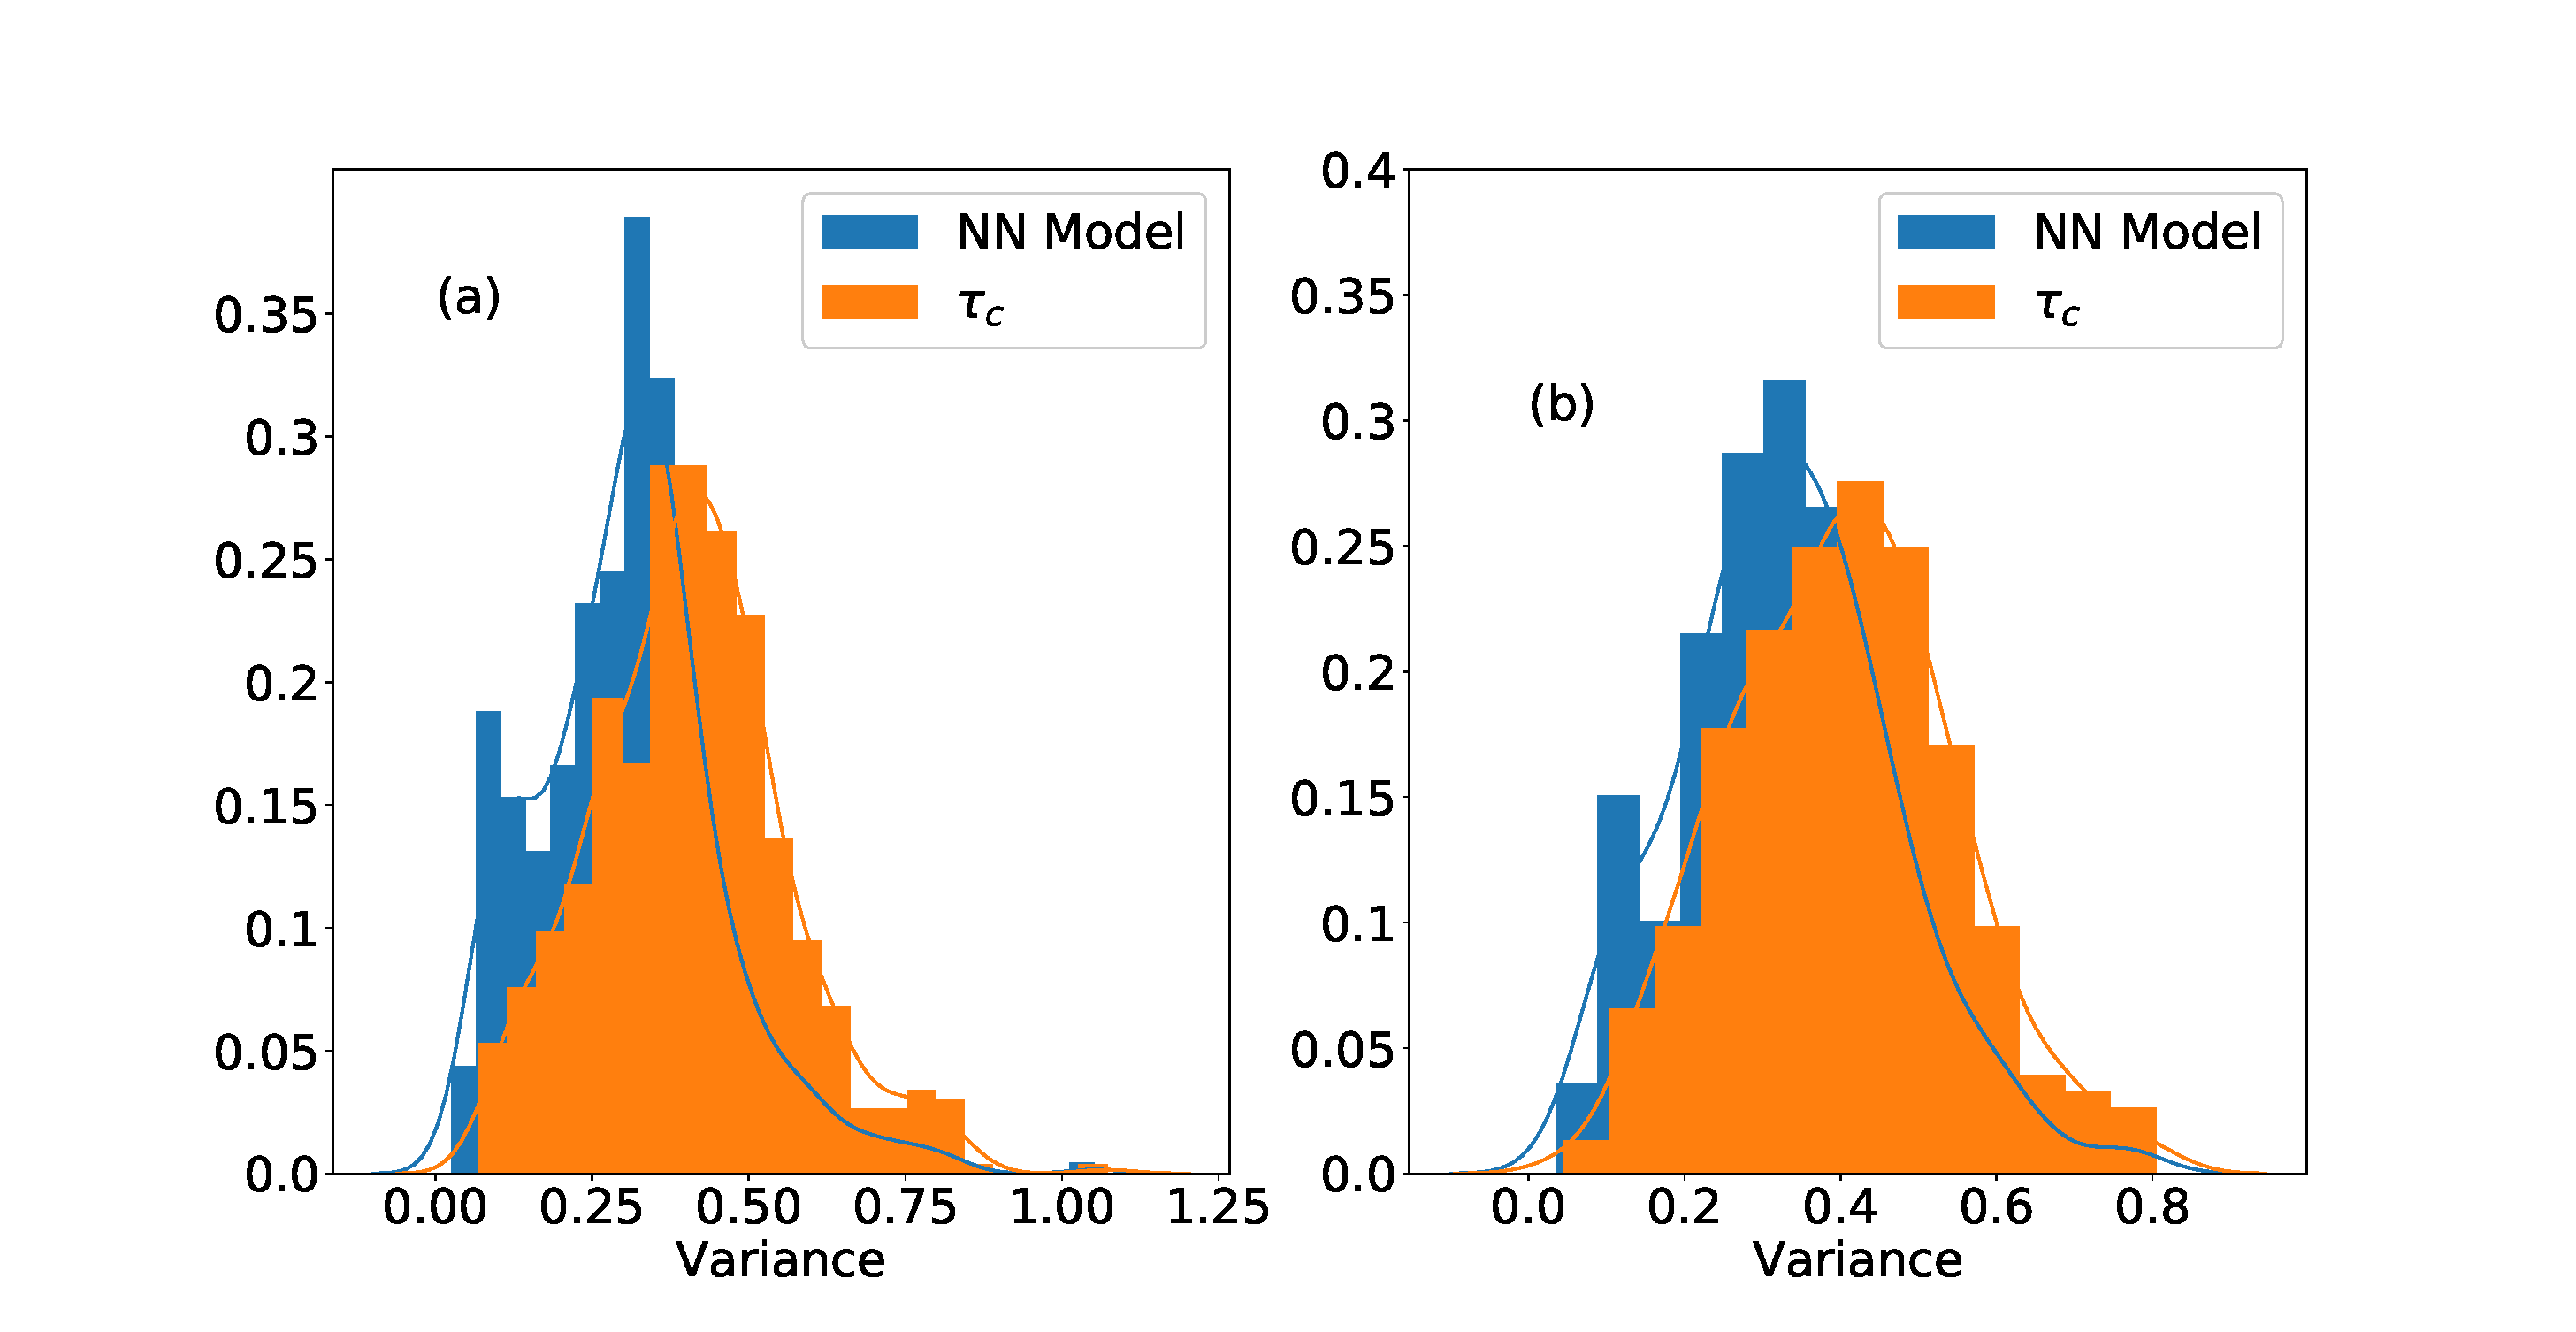
\includegraphics[width=\linewidth]{img/9.eps} 
 \renewcommand{\figurename}{图} 
\caption{单一事件预估方差分布。横轴为方差大小,纵轴为该方差的密度。\\
(a) 截至震级为4级K方法与NN模型方差分布;\\
(b) 截至震级为3级K方法与NN模型方差分布} 
%英文标题begin 
\addtocounter{figure}{-1} \vspace{-5pt} 
%\SetEnglishCaption 
\renewcommand{\figurename}{Fig} 
\caption{Single event estimation variance distribution. The horizontal axis is the variance and the vertical axis is the density of the variance.\\
(a) The Kanamori method and the NN model variance distribution up to the
magnitude 4; \\
(b) The Kanamori method and the NN model variancedistribution up to the magnitude 3} 
\renewcommand{\figurename}{图} 
%英文标题end 
\label{fig:network-device-influence.png} 
\end{figure}
	% 结论。
	% Copyright (c) 2008-2009 solvethis
% Copyright (c) 2010-2011 Casper Ti. Vector
% Public domain.




	\begin{appendix}
		% 参考文献。
		\nocite{*}
		\bibliography{ref/pkuthss.bib}
		
	\end{appendix}

	% 以下为正文之后的部分。
	\backmatter

	% 致谢。
	% Copyright (c) 2008-2009 solvethis
% Copyright (c) 2010-2011 Casper Ti. Vector
% Public domain.

\chapter{致谢}

\indent 感谢张海明老师两年来对我的教诲和关怀。从大三伊始,我便参加了张海明老师的组会。在这两年以来,张老师在学习和研究中给予了我诸多指导,让我能够有机会了解和接触到学术研究工作。无论是在本文的研究中,还是在本科生科研的研究中,张老师都花费了巨大的心血来指导我的工作。在学术上,张老师秉承严谨的作风。对于研究,无论是在实质内容上,还是展示的形式,张老师对于我们都是严格要求。因此,虽然现在的学术研究水平仍然非常有限,但是在张老师的严格要求之下,也能看到自己的进步。除此之外,张老师对于自我价值的坚持,和对于学术最本质的热爱也让人敬佩不已。\\
\indent 此外,还要感谢研究小组的冯禧师兄,和钱峰师兄。在和他们讨论的过程中给我很多思路和灵感,同时在该论文完成的过程中,两位师兄也给予了诸多的建议。同时,师兄们对于学术和知识的追求以及对于研究工作认真、刻苦的精神,时刻激励着我。\\
\indent 感谢本科期间所有的老师。四年来是你们让我从一个懵懂的少年成长为了一位具备一定的基础知识,具有初步科研能力的成熟大学生。在燕园4年的课堂上,我不仅得到了知识的提升,更是能力,认知,思想的进步。\\
\indent 感谢我的室友卢思奇,姜鹏飞,龚旭日。大学四年,无论是在学习上,还是在生活中,都受到了他们的诸多关照。感谢向直柳大学四年的陪伴,在我困惑迷茫之时给予了我很多安慰。感谢各位同学,朋友在大学四年的陪伴以及给予我的帮助。\\
\indent 最后要感谢我的父母和家人。是你们对我全力的理解和支持让我能够全力以赴在这求学之旅上前行。
	% 原创性声明和使用授权说明。
	\include{chap/originauth}
\end{document}

